%%
%% viQuantAgent / QuantAgent VN -- Academic Paper
%% Converted to the Elsevier elsarticle (numbered-citation) template,
%% based on elsarticle-template-num.tex, for submission to
%% Expert Systems with Applications (ESWA).
%%
%% FORMAT CONVERSION ONLY: the scientific content is unchanged from the
%% original cas-sc source (DKE_2026.tex); only front-matter markup and
%% class-specific macros (\credit, \printcredits, [pos=...] float
%% placement, \begin{keywords}, \tnotemark/\fnmark/\cormark, natbib
%% \citep) have been adapted to elsarticle conventions.
%%
\documentclass[preprint,12pt]{elsarticle}

\usepackage[
    left=1.8cm,
    right=1.8cm,
    top=2.0cm,
    bottom=2.0cm
]{geometry}

%% Use the option review to obtain double line spacing
%% \documentclass[authoryear,preprint,review,12pt]{elsarticle}

%% Use the options 1p,twocolumn; 3p; 3p,twocolumn; 5p; or 5p,twocolumn
%% for a journal layout -- left commented, preprint style is used here.
%% \documentclass[final,3p,times]{elsarticle}

%% For including figures, graphicx.sty has been loaded in elsarticle.cls.

%% The amssymb package provides various useful mathematical symbols
\usepackage{amssymb}
%% The amsmath package provides various useful equation environments.
\usepackage{amsmath}

%% Packages required by the original manuscript content (tables,
%% algorithms, float placement) -- preserved from the source document.
\usepackage[T1]{fontenc}
\usepackage[utf8]{inputenc}
\usepackage[vietnamese, english]{babel}
\usepackage{xcolor}
\usepackage{amsmath}
\usepackage{graphicx}
\usepackage{tabularx}
\usepackage{float}
\usepackage{placeins}
\usepackage{framed}
\usepackage[ruled,vlined,linesnumbered]{algorithm2e}
\usepackage{orcidlink}

\journal{Expert Systems with Applications}

%% Figures live under figures/figs/... in this project; original
%% \includegraphics calls use the relative path "figs/..." as in the
%% source manuscript, so we add "figures/" to the graphics search path.
\graphicspath{{figures/}}

\begin{document}

\begin{frontmatter}

%% Title, authors and addresses

\title{A Multi-Agent Large Language Model Approach to Price-Driven Stock Trading in the Vietnamese Stock Market\tnoteref{t1}}
\tnotetext[t1]{This research is funded by Foreign Trade University under research program number FTURP02-2026-08.}

%% Authors
\author[1]{Hong-Viet Tran\,\orcidlink{0000-0002-4675-2123}}
\author[1]{Hoang-Dung Phan\,\orcidlink{0009-0003-6859-0852}}
\author[1,2]{Thanh-Tam Do Thi\,\orcidlink{0000-0002-7594-276X}}
\author[1]{Phuong-Thai Nguyen\,\orcidlink{0009-2063-7338-7789}}
\author[3]{Van-Tang Nguyen\,\corref{cor1}\orcidlink{0009-0009-7266-2437}}

%% Affiliations
\affiliation[1]{organization={Institute for Artificial Intelligence, University of Engineering and Technology, Vietnam National University},
            city={Hanoi},
            country={Vietnam}}

\affiliation[2]{organization={Faculty of Economic Information System and E-Commerce, Thuongmai University},
            city={Hanoi},
            country={Vietnam}}

\affiliation[3]{organization={Faculty of Technology and Data Science, Foreign Trade University},
            city={Hanoi},
            country={Vietnam}}

\cortext[cor1]{Corresponding author}


%% Abstract
\begin{abstract}
Algorithmic trading research increasingly uses large language models (LLMs), yet most systems assume liquid, English-dominated markets. We present a five-agent LangGraph system for Vietnamese equities that combines technical indicators, point-in-time selection from 85 OHLCV alpha candidates, Vietnamese sentiment context, vision-language chart analysis, and a binary LONG/SHORT decision. A paired shared-report protocol holds Indicator, Pattern, and Trend evidence fixed between Full and No-Alpha branches, while a fixed-cycle long-only ledger compounds wealth and charges fee and slippage on both transaction legs. Across nine equities and 180 paired test points, Full accuracy is 65.0\% versus 51.1\% for No-Alpha, a mean lift of 13.9 percentage points (cross-symbol Wilcoxon $p=0.0078$). Mean Full account return remains negative at $-1.69\%$, so directional improvement does not imply profitability. A four-way ablation on FPT, VNM, and VCB attributes a larger independent contribution to alpha factors (+8.33 pp on average) than sentiment (+1.67 pp) and reveals heterogeneous interactions.
\end{abstract}

%%Graphical abstract
\begin{graphicalabstract}
\centering
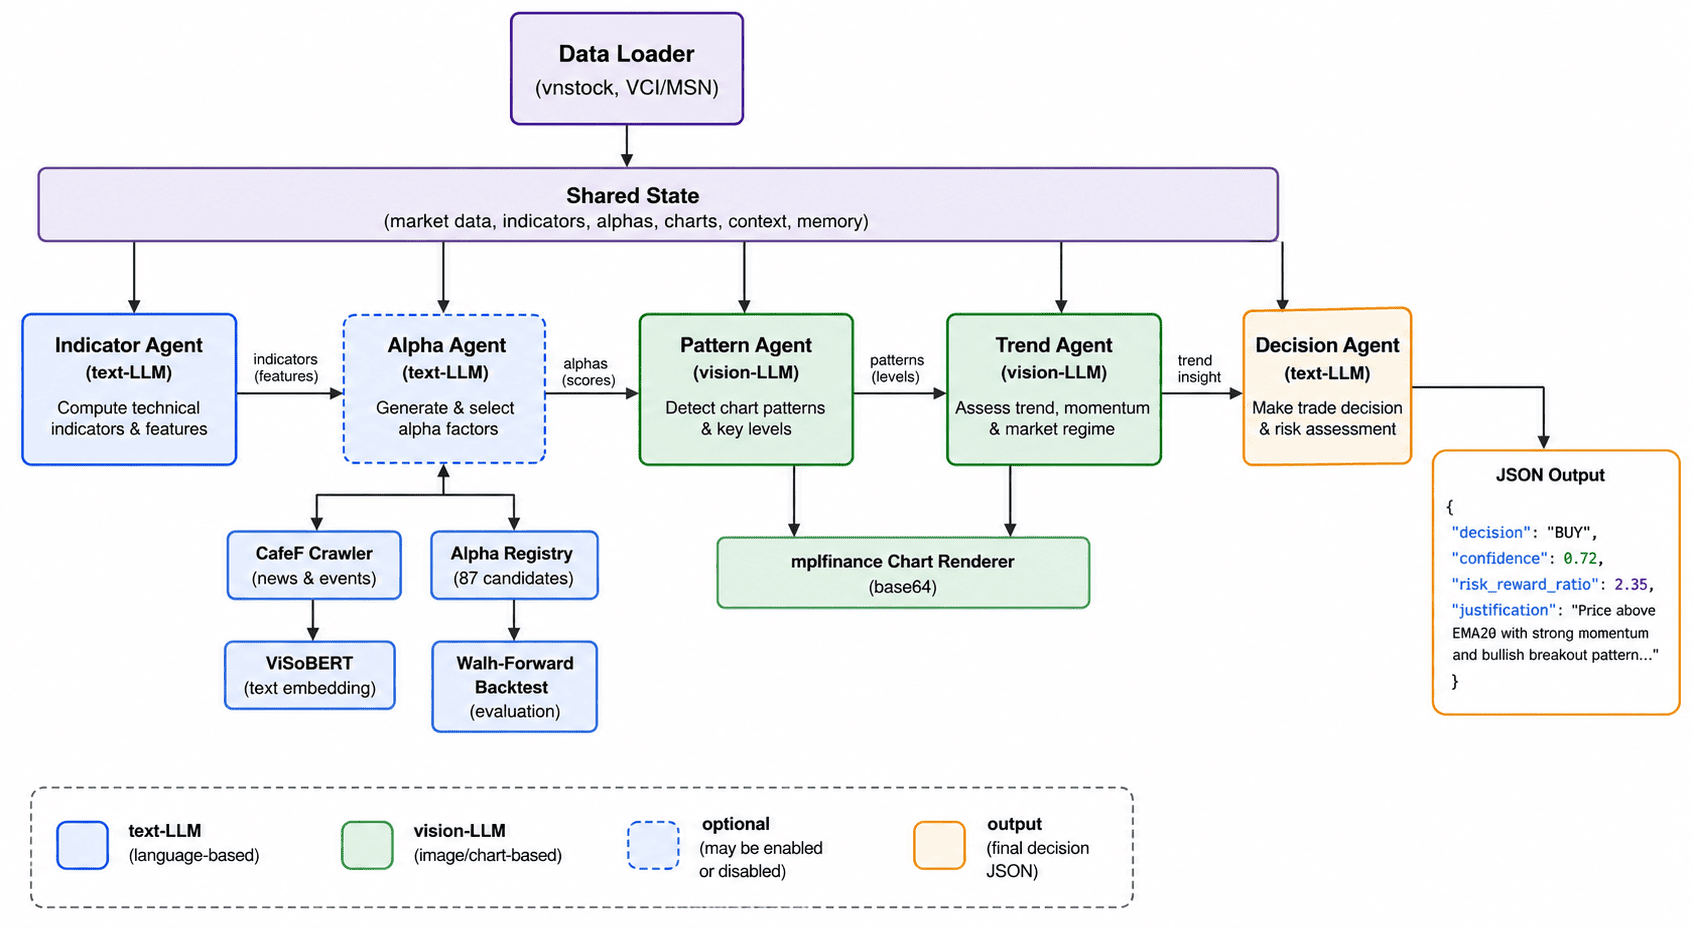
\includegraphics[width=0.95\textwidth]{figs/system_pipeline.png}
\end{graphicalabstract}

%%Research highlights
\begin{highlights}
\item A leakage-safe five-agent LangGraph system for Vietnamese equities.
\item Paired shared reports isolate the Alpha bundle on 180 test points.
\item Full accuracy reaches 65.0\% versus 51.1\% for No-Alpha.
\item A compounded long-only ledger separates accuracy from economic return.
\item Four-way ablation disentangles alpha factors and sentiment context.
\end{highlights}

%% Keywords
\begin{keyword}
Multi-agent LLM \sep Vietnamese stock market \sep Alpha factor selection \sep Sentiment analysis
\end{keyword}

\end{frontmatter}
% The elsarticle preprint footer exceeds its output box by 2.61pt.
% Visual inspection confirms no clipping; use a 3pt output tolerance.
\global\hfuzz=3pt

%% main text
\section{Introduction}

Large language models (LLMs) have recently shown strong potential as reasoning engines in financial analysis, enabling multi-agent systems to coordinate over heterogeneous signals-price data, technical indicators, chart patterns, and news sentiment-within a unified pipeline. While frameworks such as QuantAgent \cite{xiong2025quantagent} establish a compelling blueprint for LLM-driven trading agents, they are designed for mature, English-language markets and do not generalize to the constraints of emerging economies.

Vietnam's equity market presents three challenges that require explicit adaptation. First, a predictive bar horizon and the assumptions of an executable cash-equity simulation are distinct; calendar gaps and instrument scope make them non-interchangeable. Second, the dominant financial news source, CafeF, publishes exclusively in Vietnamese, making English-centric sentiment pipelines inapplicable. Third, the shallow cross-sectional universe of HOSE, HNX, and UPCoM calls for alpha factor selection methods suited to single-stock Open, High, Low, Close, and Volume (OHLCV) data rather than the large-universe assumptions of standard factor libraries.

We present a five-agent LangGraph \cite{langgraph2024} pipeline that addresses each of these gaps. An Alpha Agent dynamically selects the top-five factors from an executable registry of exactly 85 candidates: five proprietary OHLCV formulas and 80 single-stock adaptations drawn from the WorldQuant 101 catalogue \cite{kakushadze2016formulaic}. Candidates are ranked by point-in-time Information Coefficient (IC), accuracy, and a Sharpe diagnostic. This accounting is important: the registry contains neither 87 candidates nor all 101 WorldQuant expressions. The factor values and ranking use OHLCV only. CafeF sentiment is supplied separately as textual context for qualitative LLM comparison. The primary configured scorer is a hosted ViSoBERT \cite{nguyen2023visobert} endpoint, with a deterministic lexicon fallback; the scorer and fallback status are recorded per article, and a run is attributed to the endpoint only when its included articles verify that path. Pattern and Trend agents apply vision-language analysis to candlestick and trendline charts, while a Decision Agent synthesises all reports into a binary LONG/SHORT direction forecast whose account action is resolved separately.

The primary objective of this paper is to evaluate whether the Alpha Agent improves directional forecasting relative to a no-alpha baseline. Indicator, Pattern, and Trend reports are generated once at each cutoff and cloned into both decision branches, providing paired common-support estimates without upstream variation inside a comparison. The nine-symbol benchmark reports directional, statistical, and compounded-account outcomes. A separate four-way shared-upstream experiment then evaluates Full, Alpha-only, Sentiment-only, and Baseline variants, allowing the factor and sentiment contributions to be distinguished rather than treating the Alpha bundle as indivisible.

The remainder of this paper is organised as follows. Section 2 reviews related work on LLM-based trading agents, Vietnamese NLP, and quantitative alpha research. Section 3 formalises the problem. Section 4 describes the system architecture. Section 5 presents the experimental setup. Section 6 reports backtest results. Section 7 discusses limitations, and Section 8 concludes.

\section{Related works}
\label{sec:relatedworks}
\subsection{LLM Agents in Financial Analysis}

The application of LLMs to financial tasks has grown rapidly, spanning earnings call analysis, financial question answering, and report summarisation. FinGPT \cite{yang2023fingpt} and BloombergGPT \cite{wu2023bloomberggpt} demonstrate that domain-adapted language models outperform general-purpose ones on financial benchmarks. More relevant to our work, TradingAgent \cite{tradingagents2024} and QuantAgent frame trading as a multi-step reasoning problem, delegating sub-tasks-market perception, reflection, and decision-to coordinated LLM agents. Our framework builds directly on this paradigm but extends it with vision-language chart analysis, quantitative alpha integration, and emerging-market adaptations absent from prior systems.

\subsection{Technical Analysis and Pattern Recognition}

Automating technical analysis has been explored through convolutional neural networks for candlestick pattern recognition \cite{tsantekidis2017candlestick}, reinforcement learning for indicator-based policy learning \cite{deng2016rltrading}, and hybrid rule-based systems \cite{lo2000technical}. Recent work has begun replacing handcrafted features with multimodal chart-understanding models. ChartLlama \cite{han2023chartllama} shows that vision-language models can extract actionable insights from charts without explicit feature engineering. Our system employs this capability within two dedicated vision agents, integrating it into a broader multi-agent decision pipeline rather than treating it in isolation.

\subsection{Quantitative Alpha Factor Research}

Systematic factor construction has a long tradition in quantitative finance, from foundational momentum and value factors \cite{jegadeesh1993momentum,fama1992crosssection} to the large-scale formulaic approach of Kakushadze, who codified 101 analytic alpha expressions (WorldQuant 101). Subsequent work adapts these formulas to single-asset settings \cite{kang2021singleasset} and evaluates their decay and capacity in different market regimes \cite{harvey2016,novy2016alpha}. However, traditional factor mining is notoriously susceptible to data-snooping and selection bias, pitfalls extensively documented by Harvey, Liu, and others. While modern non-LLM multimodal pipelines attempt to mitigate this by fusing factors with alternative data via standard machine learning architectures, they often lack the explicit semantic reasoning needed to contextualize anomalies. We extend this literature by constructing an 85-candidate registry-combining the full WorldQuant 101 corpus adapted to single-stock OHLCV with five proprietary formulas-and selecting the top-five factors per symbol dynamically via walk-forward Information Coefficient and Sharpe ratio ranking.

\subsection{Sentiment Analysis in Finance and Vietnamese NLP}

News sentiment has been established as a statistically significant predictor of short-term price movements \cite{tetlock2007news}, with transformer-based models such as FinBERT \cite{araci2019finbert} setting the standard for English financial text. For Vietnamese, ViSoBERT provides a BERT-based model pre-trained on large-scale Vietnamese corpora and achieves strong results on Vietnamese sentiment classification benchmarks. Financial-domain validity does not follow automatically from general-language benchmark performance. We therefore configure a hosted ViSoBERT endpoint as the primary scorer while retaining an explicit lexicon fallback, and record the actual scoring path for every newly scored article. Target and related-company sentiment are presented in a separate LLM text context and do not enter the OHLCV factor formulas or ranking. Legacy cache entries that lack scorer metadata are treated as unknown rather than retrospectively attributed to ViSoBERT.

\subsection{Trading Systems for Emerging Markets}

Research on algorithmic trading in emerging markets is comparatively sparse. Studies on the Vietnamese market have primarily examined market efficiency \cite{vo2019efficiency}, herding behaviour \cite{pham2021herding}, and the predictive power of classical technical indicators under the price-limit regime \cite{truong2020technical}, but none employs LLM-based agents. Our work develops a multi-agent LLM forecasting framework that records Vietnamese cash-equity execution and settlement assumptions separately from the domestic news ecosystem and single-stock OHLCV data characteristics; we do not claim that a universal settlement rule fixes a model horizon.

\subsection{Evaluation Standards and Agentic Benchmarks}

Recent literature highlights the critical need for rigorous, standardized evaluation in LLM-driven trading. For instance, FinVision \cite{fatemi2024finvision} shares our modular multi-agent approach and vision-based technical analysis but places much stronger emphasis on extensive ablations (e.g., of reflection modules) and comprehensive risk reporting (Sharpe, drawdowns). Furthermore, an audit-oriented survey on financial LLMs \cite{xia2026agentictrading} identifies widespread methodological gaps in time-consistent splits, transaction-cost modeling, and reproducibility. While our framework addresses costs and lookahead leakage, we recognize that our reporting detail currently falls short of the rigorous bar for full reproducibility. Finally, live/prediction-market benchmarks \cite{zhang2026predictionarena, arora2026predictionmarketbench} and forward-looking evaluation paradigms like FutureX \cite{zeng2025futurexadvancedlivebenchmark} underscore that static walk-forward backtests--while useful--must ultimately be complemented by live trials and execution realism to substantiate strong claims about agentic efficacy.

\section{Problem Formulation}
\label{sec:formulation}

\begin{algorithm}[htbp]
\small
\caption{Walk-Forward Evaluation}
\label{alg:walkforward}

\KwIn{
OHLCV series $\mathbf{X}$,
alpha registry $\mathcal{A}$,
historical sentiment cache $\mathcal{D}$,
window size $W$,
lookahead $L$,
step size $S$
}

\KwOut{
Directional predictions $\hat{y}_{e,L}$,
accuracy, Alpha Lift, and compounded account return
}

Initialize results list $\mathcal{R} \leftarrow \emptyset$

\ForEach{test point $e$ in the walk-forward schedule}{

    Extract the exact analysis window $\mathbf{X}_e=\mathbf{X}_{[e-W,e)}$

    Compute technical indicators using TA-Lib

    Evaluate all candidate alphas $\alpha^{(k)} \in \mathcal{A}$

    Remove candidates with no fitted transform, fewer than 20 finite
    evaluation observations, or non-finite ranking metrics to form $\mathcal{V}$

    Min--max normalise each metric over $\mathcal{V}$ and rank using:

    \[
    S_k =
    0.40\mathcal{N}_{\mathcal{V}}(|IC_k|)
    + 0.35\mathcal{N}_{\mathcal{V}}(Acc_k)
    + 0.25\mathcal{N}_{\mathcal{V}}(Sharpe_k)
    \]

    Select top-5 alpha factors $\mathcal{A}^{*}$

    Retrieve historical CafeF sentiment at the decision cutoff $d=e-1$

    Generate candlestick and trendline chart images from the same exact
    $\mathbf{X}_e$ window

    Run the Indicator, Alpha, Pattern, and Trend Agents

    Pass all reports to Decision Agent

    Obtain binary prediction
    $\hat{y}_{e,L} \in \{\texttt{LONG}, \texttt{SHORT}\}$

    Compare prediction with realised return

    Store metrics in $\mathcal{R}$
}

Compute directional accuracy and Alpha Lift

Compute compounded account return under Eq.~\eqref{eq:account_return}

\Return{$\mathcal{R}$}

\end{algorithm}
\subsection{Market Model and Data}

Let $\mathcal{S} = \{s_1, s_2, \ldots, s_N\}$ denote the universe of
Vietnamese equities listed on HOSE, HNX, or UPCoM.
For each asset $s \in \mathcal{S}$, the market is observed as a
discrete-time OHLCV series:
\begin{equation}
    \mathbf{x}_u = \bigl(O_u,\, H_u,\, L_u,\, C_u,\, V_u\bigr)
    \;\in\; \mathbb{R}^5_{+},
    \quad u = 0, 1, \ldots, T-1,
\end{equation}
where $O_u$, $H_u$, $L_u$, $C_u$, $V_u$ denote the open, high, low,
closing price, and trading volume at zero-based bar position $u$ respectively.
When volume observations are missing for more than 50\% of bars, the
intra-bar range $H_u - L_u$ is substituted as a liquidity proxy.

We use zero-based row positions and an exclusive window-end boundary.  For a
test point with boundary $e$, the analysis window of size $W$ is exactly:
\begin{equation}
    \mathbf{X}_{e} = \bigl(\mathbf{x}_{e-W},\,
                           \mathbf{x}_{e-W+1},\, \ldots,\,
                           \mathbf{x}_{e-1}\bigr)
    \;\in\; \mathbb{R}^{W \times 5}.
    \qquad\text{(equivalently, }\mathbf{X}_{e}=\mathbf{X}_{[e-W,e)}\text{)}
\end{equation}
Thus $e$ is not itself a visible bar: the final visible (decision) bar is
$d=e-1$.  The next bar, $e$, is reserved for the earliest simulated entry,
and the immutable label target is $h=e-1+L$.  A candidate economic exit may
use that close only if the separate execution contract accepts it. This mapping is used in the
engine, alpha labels, persisted provenance, and the experiments:
\begin{equation}
    \boxed{\quad
    \text{window}=[e-W,e),\qquad d=e-1,\qquad
    \text{entry}=e,\qquad h=e-1+L.\quad}
    \label{eq:time_index_contract}
\end{equation}
The mapping is positional rather than calendar arithmetic; timestamps are
carried alongside every index, so a weekend or holiday gap does not create a
synthetic bar.  The first complete window is $e=W$, and it is evaluable only
when the target is present, i.e., $T\geq W+L$.  For $L=1$, the target is the
entry bar ($h=e$), while for $L=3$ it is two positions after entry
($h=e+2$).  Any boundary whose target is outside the available frame is
rejected rather than shortened.

\subsection{Directional Prediction Task}

The core task predicts whether a candidate LONG cycle is profitable after
the configured transaction costs. With $d=e-1$ and $h=e-1+L$, define
\begin{equation}
    r^{\mathrm{net}}_{e,L}
    =\frac{C_h}{O_e}
      \frac{(1-c_{\mathrm{slip}})(1-c_{\mathrm{fee}})}
           {(1+c_{\mathrm{slip}})(1+c_{\mathrm{fee}})}-1,
    \qquad
    y_{e,L}=
    \begin{cases}
        +1, & r^{\mathrm{net}}_{e,L}>0,\\
        -1, & r^{\mathrm{net}}_{e,L}\leq 0.
    \end{cases}
    \label{eq:label}
\end{equation}
Here $O_e$ is the next-bar entry open and $C_h$ is the target close. The same
net Open-to-Close return defines the directional label, the alpha-selection
target, and the realised return of an executed LONG. Thus an opening gap and
both transaction legs are represented consistently. The reported study uses
daily bars with $L=3$; intraday execution is outside its empirical scope.

A trading system $\mathcal{F}$ maps each analysis window to a binary
decision:
\begin{equation}
    \hat{y}_{e,L} \;=\; \mathcal{F}\!\bigl(\mathbf{X}_e\bigr)
    \;\in\; \{-1,\, +1\},
\end{equation}
where $+1$ corresponds to a \texttt{LONG} signal and $-1$ to
\texttt{SHORT}.

\subsection{Alpha Factor Formalisation and Adaptation}

An \emph{alpha factor} $\alpha^{(k)}$ is a measurable function that maps
a feature frame derived from $\mathbf{X}_e$ to a scalar signal:
\begin{equation}
    \alpha^{(k)} : \mathbb{R}^{T_{\mathrm{hist}} \times d}
    \;\longrightarrow\; \mathbb{R},
\end{equation}
where $d$ is the number of engineered features and
$T_{\mathrm{hist}}$ is the historical window used for computation.

The executable registry contains 80 adaptations drawn from the WorldQuant-101 catalogue, not all 101 source expressions, plus five proprietary formulas. The source expressions were designed primarily for cross-sectional ranking across a broad, liquid equity universe. To apply the registered subset to a single Vietnamese stock, we use a \emph{semantic translation layer} that replaces cross-sectional operators with rolling time-series surrogates. This is an engineering heuristic rather than an invariance-preserving mathematical transformation.

\paragraph{Operator Localisation.}
The primary transformation involves the cross-sectional $\operatorname{rank}(x)$ operator, which denotes the relative percentile of a stock against its peers. A cross-sectional rank is localised to a 20-bar time-series percentile rank unless the source expression already specifies a time-series rank with its own window. Let $\mathcal{H}_{u,w}$ contain the available preceding observations in that rolling window and let $n_{u,w}=|\mathcal{H}_{u,w}|+1$. The implementation computes
\begin{equation}
    \operatorname{ts\_rank}(x_u,w)
    \;=\;
    \frac{1}{\max(n_{u,w}-1,1)}
    \sum_{x_v\in\mathcal{H}_{u,w}} \mathbf{1}[x_u>x_v].
    \label{eq:ts_rank_localised}
\end{equation}
Thus ties are not counted as strictly lower values, and an initial partial window is permitted once the operator-specific minimum is met. Other explicit time-series lookbacks are retained from each registered expression and can be substantially longer than 20 bars. Average Daily Volume ($\mathrm{ADV}_{n}$) is the asset's own $n$-day rolling mean volume, and VWAP is approximated by the daily typical price $(H_u+L_u+C_u)/3$. Functions $\delta(x,d)$ and $\operatorname{delay}(x,d)$ are implemented as $d$-period differences and lags. These substitutions remove peer-relative information, so neither the economic interpretation nor the stochastic properties of the source cross-sectional alpha are presumed to survive unchanged.

\paragraph{Consistent Normalisation.}
To ensure comparability across candidates with different scales, each adapted raw alpha value is normalised to $[-1,1]$ via:
\begin{equation}
    \tilde{\alpha}^{(k)}_{u,e}
    \;=\;
    \tanh\!\left(
        \frac{\alpha^{(k)}_u - \mu_{k,e}}{\sigma_{k,e} + \varepsilon}
    \right),
    \label{eq:alpha_norm}
\end{equation}
where $\mu_{k,e}$ and $\sigma_{k,e}$ are computed over the finite values in
the cutoff-safe calibration snapshot available at decision boundary $e$, and
$\varepsilon > 0$ prevents division by zero. They are recomputed at the next
cutoff; they are not estimated from the entry or target bars.
The resulting signal $\tilde{\alpha}^{(k)}_u \in (-1, 1)$ is treated as
a continuous directional score: positive values favour \texttt{LONG} and
negative values favour \texttt{SHORT}.

\subsection{Walk-Forward Alpha Selection}

Let $\mathcal{A} = \bigl\{\alpha^{(1)}, \alpha^{(2)}, \ldots,
\alpha^{(M)}\bigr\}$ denote the registry of $M = 85$ candidate alpha
functions. Each point-in-time history ends at the decision cutoff and is
therefore disjoint from the current entry and target bars. Given the net
Open-to-Close execution-return series $r^{\mathrm{net},(L)}_u$ defined as in
Eq.~\eqref{eq:label}, the following diagnostics are computed on finite
historical observations:

The same matured calibration sample is used to estimate IC sign, orient the
signal, calculate the three ranking diagnostics, and select the top five.
Consequently, point-in-time truncation prevents future-data leakage but does
not provide an independent inner/outer assessment of the adaptive selection
rule. The equations below define the implemented selector; they should not be
read as post-selection-unbiased estimates of an individual factor's skill.

\paragraph{Information Coefficient (IC).}
Following Grinold and Kahn \cite{grinold1999active}, the Spearman rank correlation between the normalised alpha signal and
forward returns over the evaluation suffix:
\begin{equation}
    \mathrm{IC}_k \;=\;
    \operatorname{SpearmanCorr}\!\bigl(
        \tilde{\alpha}^{(k)}_{\mathcal{T}_{\mathrm{eval}}},\;
        r^{\mathrm{net},(L)}_{\mathcal{T}_{\mathrm{eval}}}
    \bigr).
    \label{eq:ic}
\end{equation}

\paragraph{Directional Accuracy.}
The fraction of bars where the predicted direction agrees with the
realised direction, restricted to bars with a strong enough signal:
\begin{equation}
    \mathrm{Acc}_k \;=\;
    \frac{1}{|\mathcal{T}^*|}
    \sum_{u \in \mathcal{T}^*}
    \mathbf{1}\!\left[
        \operatorname{sign}\!\bigl(\tilde{\alpha}^{(k)}_u\bigr)
        = y^{(L)}_u
    \right],
\end{equation}
where $\mathcal{T}^* = \bigl\{u : |\tilde{\alpha}^{(k)}_u| > 0.05\bigr\}$
excludes near-zero signals and $y^{(L)}_u$ is the canonical binary label from
Eq.~\eqref{eq:label}; hence a zero net return is \texttt{DOWN}, not a third class.

\paragraph{Long-Only Win Rate.}
The precision of the alpha on bullish signals:
\begin{equation}
    \mathrm{LongAcc}_k \;=\;
    \frac{
        \sum_u \mathbf{1}\!\left[
            \tilde{\alpha}^{(k)}_u > 0.05 \;\wedge\; r^{\mathrm{net},(L)}_u > 0
        \right]
    }{
        \sum_u \mathbf{1}\!\left[
            \tilde{\alpha}^{(k)}_u > 0.05
        \right]
    }.
\end{equation}

\paragraph{Horizon Sharpe diagnostic.}
For ranking, define $z^{(k)}_u=\operatorname{sign}(\tilde{\alpha}^{(k)}_u)
r^{\mathrm{net},(L)}_u$ on the finite historical sample. Following Sharpe
\cite{sharpe1966mutual}, the diagnostic is:
\begin{equation}
    \mathrm{Sharpe}_k \;=\;
    \sqrt{\frac{252}{L}} \cdot
    \frac{
        \mathbb{E}_{u\in\mathcal{T}_{\mathrm{eval}}}\!\left[z^{(k)}_u\right]
    }{
        \mathrm{Std}_{u\in\mathcal{T}_{\mathrm{eval}}}\!\left[z^{(k)}_u\right]
        + \varepsilon
    }.
    \label{eq:sharpe}
\end{equation}
Sortino, maximum drawdown, hit rate, long-only accuracy, and average trade are
retained as descriptive candidate diagnostics but do not enter the composite
selection score.

Candidates with no fitted transform, fewer than 20 finite evaluation
observations, or a non-finite value for any ranking metric are excluded before scaling. Let
$\mathcal{V}\subseteq\mathcal{A}$ be the remaining eligible set and let
$q\in\{|\mathrm{IC}|,\mathrm{Acc},\mathrm{Sharpe}\}$.
The implementation applies candidate-wise min--max scaling:
\begin{equation}
    \mathcal{N}_{\mathcal{V}}(q_k) =
    \begin{cases}
        \dfrac{q_k-q_{\min}}{q_{\max}-q_{\min}},
        & q_{\max}-q_{\min} \geq \varepsilon_{\mathrm{rank}},\\[6pt]
        \dfrac{1}{2}, & \text{otherwise},
    \end{cases}
    \label{eq:candidate_minmax}
\end{equation}
where $q_{\min}=\min_{j\in\mathcal{V}}q_j$,
$q_{\max}=\max_{j\in\mathcal{V}}q_j$, and
$\varepsilon_{\mathrm{rank}}=10^{-9}$. The default composite selection
score is therefore:
\begin{equation}
    S_k \;=\;
    0.40\,\mathcal{N}_{\mathcal{V}}(|\mathrm{IC}_k|)
    \;+\; 0.35\,\mathcal{N}_{\mathcal{V}}(\mathrm{Acc}_k)
    \;+\; 0.25\,\mathcal{N}_{\mathcal{V}}(\mathrm{Sharpe}_k).
    \label{eq:composite}
\end{equation}

The weights prioritise association and directional accuracy while retaining a
risk-adjusted return diagnostic. Long-only accuracy is reported but excluded
from ranking to avoid favouring factors solely because the sample trends up.

Signal orientation is inferred from the sign of IC on the cutoff-safe
historical snapshot. A negative-IC candidate is multiplied by $-1$ for its
historical directional metrics and for the current inference value. All labels
used for this operation have matured by the decision cutoff, but estimating
orientation and ranking on the same finite history remains a selection risk
discussed in Section~\ref{sec:limitations_futurework}.

Let $K=\min(5,|\mathcal{V}|)$. The top candidates are selected as:
\begin{equation}
    \mathcal{A}^{*} \;=\;
    \underset{\mathcal{B}\,\subseteq\,\mathcal{V},\;|\mathcal{B}|=K}
    {\arg\max}
    \;\sum_{\alpha^{(k)} \in \mathcal{B}} S_k.
    \label{eq:selection}
\end{equation}

\subsection{Sentiment Signal Construction}

Let $\mathcal{D}_e = \{d_1, d_2, \ldots, d_{|\mathcal{D}_e|}\}$ be the
set of CafeF articles available to the system for asset $s$ at the timestamp
$\tau_d$ of decision bar $d=e-1$.
Each article is assigned a score by the scorer actually recorded for that
article:
\begin{equation}
    \rho_i \;=\; \mathrm{Scorer}_i(d_i) \;\in\; [-1,\, 1],
\end{equation}
where $\rho_i = +1$ denotes strongly positive, $-1$ strongly negative,
and $0$ neutral sentiment. For newly scored records,
$\mathrm{Scorer}_i$ is either the configured
\texttt{5CD-AI/Vietnamese-Sentiment-visobert} HF Inference API endpoint or
the versioned deterministic lexicon fallback. Each record stores the scorer,
requested model identifier, observed Hub revision and its verification status,
and fallback status/reason. Legacy scores without these fields are marked
\texttt{legacy-unknown}; no model identity is inferred from their numeric values.

The unweighted mean sentiment score for descriptive reporting is:
\begin{equation}
    \bar{\rho}_e \;=\;
    \frac{1}{|\mathcal{D}_e|} \sum_{i=1}^{|\mathcal{D}_e|} \rho_i.
\end{equation}

For the causal sentiment context, each dated article receives an exponential
weight based on its age at cutoff $\tau_d$:
\begin{align}
    \Delta_i(\tau_d) &= \tau_d - \mathrm{date}(d_i), \\
    w_i(\tau_d) &= 2^{-\Delta_i(\tau_d)/h}, \qquad h=30\ \text{days}, \\
    S_{\mathrm{decay},e}
    &= \frac{\sum_{d_i\in\mathcal{D}_e} w_i(\tau_d)\rho_i}
             {\sum_{d_i\in\mathcal{D}_e} w_i(\tau_d)},
    \label{eq:sent_decay} \\[4pt]
    \mathrm{Rel}_{\mathrm{sent},e}
    &\;=\;
    S_{\mathrm{decay},e} \;-\;
    \frac{1}{|\mathcal{R}_e|}
    \sum_{s' \in \mathcal{R}_e} S^{(s')}_{\mathrm{decay},e},
    \label{eq:relsent}
\end{align}
where $\mathcal{R}_e$ contains only related companies with at least three
valid dated-and-scored articles at cutoff $\tau_d$.  The exponential mean makes recent articles
more influential without comparing a batch mean against the same batch from
which it was calculated.  $\mathrm{Rel}_{\mathrm{sent},e}$ compares like-for-like
time-decayed scores.

\paragraph{Batch definition and low-news stability.}
The set $\mathcal{D}_e$ contains all dated articles for target stock $s$ in the 90-day sliding window ending at cutoff $\tau_d$. The complete compact observation set is used for Eq.~\ref{eq:sent_decay}; the 15-article list stored for display is not the normalization sample. With fewer than three valid dated-and-scored observations, $S_{\mathrm{decay},e}$ is marked unavailable rather than assigned a neutral zero. Likewise, $\mathrm{Rel}_{\mathrm{sent},e}$ is unavailable when $\mathcal{R}_e$ is empty. The effective sample size, invalid-date/score counts, and number of post-cutoff observations excluded are stored in run provenance. Neither context variable enters any numerical alpha formula or the registry ranking.

To prevent look-ahead leakage during backtesting, every cached article stores
timezone-aware \texttt{published\_at} and \texttt{available\_at} fields in
\texttt{Asia/Ho\_Chi\_Minh}. The cache is keyed by $(s,\,\tau_d)$ and returns only
articles satisfying $\mathrm{available\_at}(d_i)\leq \tau_d$. CafeF records having
date-only precision are assigned a conservative availability time of 00:00 on
the following local day; records without a parseable date are rejected in
research mode and never used to fill a sparse historical window. All 180
articles in the nine supplied cache artifacts contain parseable dates, so the
previous undated fallback was a latent risk rather than evidence that those
reported runs actually consumed undated articles.

\subsection{Multi-Agent Decision Function}

The full system decomposes $\mathcal{F}$ into five
sub-functions corresponding to the five specialised agents:
\begin{align}
    \mathbf{r}^{\mathrm{ind}}
    &\;=\; \mathcal{F}_{\mathrm{ind}}\!\bigl(\mathbf{X}_e\bigr),
    \label{eq:ind} \\
    \mathbf{a}_e
    &\;=\; \mathcal{F}_{\mathrm{factor}}\!\bigl(
            \mathbf{X}_e,\; \mathcal{A}^{*}
           \bigr),
    \label{eq:alpha_factor} \\
    \mathbf{c}^{\mathrm{sent}}_e
    &\;=\; \mathcal{F}_{\mathrm{context}}\!\bigl(
            \mathcal{D}_e,\;
            S_{\mathrm{decay},e},\;
            \mathrm{Rel}_{\mathrm{sent},e}
           \bigr),
    \label{eq:sent_context} \\
    \mathbf{r}^{\mathrm{alpha}}
    &\;=\; \mathcal{F}_{\mathrm{text}}\!\bigl(
            \mathbf{a}_e,\; \mathbf{c}^{\mathrm{sent}}_e
           \bigr),
    \label{eq:alpha} \\
    \mathbf{r}^{\mathrm{pat}}
    &\;=\; \mathcal{F}_{\mathrm{pat}}\!\bigl(
            \mathbf{I}^{\mathrm{kline}}_e
           \bigr),
    \label{eq:pat} \\
    \mathbf{r}^{\mathrm{trend}}
    &\;=\; \mathcal{F}_{\mathrm{trend}}\!\bigl(
            \mathbf{I}^{\mathrm{trend}}_e
           \bigr),
    \label{eq:trend}
\end{align}
where $\mathbf{I}^{\mathrm{kline}}_e$ and
$\mathbf{I}^{\mathrm{trend}}_e$ are the candlestick and
trendline-annotated chart images rendered from $\mathbf{X}_e$, and
$\mathbf{c}^{\mathrm{sent}}_e$ is a separate textual context containing the
target and related-company sentiment summaries. The factor values in
$\mathbf{a}_e$ are functions of $\mathbf{X}_e$ only; the LLM compares
them qualitatively with $\mathbf{c}^{\mathrm{sent}}_e$ when producing
$\mathbf{r}^{\mathrm{alpha}}$.

The Decision Agent aggregates all four reports through structured
chain-of-thought prompting \cite{wei2022chain} and produces the final binary signal:
\begin{equation}
    \hat{y}_{e,L} \;=\; \mathcal{F}_{\mathrm{dec}}\!\bigl(
        \mathbf{r}^{\mathrm{ind}},\;
        \mathbf{r}^{\mathrm{alpha}},\;
        \mathbf{r}^{\mathrm{pat}},\;
        \mathbf{r}^{\mathrm{trend}}
    \bigr) \;\in\; \{-1,\, +1\}.
    \label{eq:decision}
\end{equation}

The forced binary output constraint ensures $\hat{y}_{e,L}\neq 0$ for every
valid \emph{prediction}; it does not imply an always-invested account. Under
the default long-only action map, \texttt{SHORT} becomes \texttt{CASH}.
\texttt{LONG} executes a complete next-open-to-target-close cycle when valid
positive prices and timestamps are available. This separation permits binary
directional evaluation without misrepresenting a bearish prediction as an
executed short sale.

\subsection{Walk-Forward Evaluation Protocol}

We adopt a rolling walk-forward evaluation protocol commonly used in quantitative trading system evaluation \cite{pardo2008evaluation}.

Given a historical series of $T$ bars, valid test points are exclusive
boundaries with $W\leq e\leq T-L$.  The implementation uses the latest
available boundaries at spacing $S$ (up to $N_{\mathrm{test}}$ points) and
processes them in chronological order:
\begin{equation}
    \mathcal{T} \;=\;
    \bigl\{\, e_i = T-L-(i-1)\cdot S
    \;\mid\; i = 1, 2, \ldots, N_{\mathrm{test}} \,\bigr\},
    \label{eq:testpoints}
\end{equation}
retaining only values $e_i\geq W$ before reversing the list for execution.
Thus $e=W$ is included whenever it is among the requested points, and every
selected point satisfies the complete-window and complete-target conditions.
Here $S$ is the step size between consecutive test points and
$N_{\mathrm{test}} = 20$ in our main experiments.

The three primary evaluation metrics are:
\begin{align}
    \mathrm{Acc}
    &\;=\;
    \frac{1}{|\mathcal{T}|}
    \sum_{e \in \mathcal{T}}
    \mathbf{1}\!\bigl[\hat{y}_{e,L} = y_{e,L}\bigr],
    \label{eq:acc} \\[4pt]
    \Delta\mathrm{Acc}
    &\;=\;
    \mathrm{Acc}_{\mathrm{Full}}
    \;-\; \mathrm{Acc}_{\mathrm{No\text{-}\alpha}},
    \label{eq:lift} \\[4pt]
    q_e
    &\;=\;
    a_e\left[
    \frac{C_{e-1+L}}{O_e}
    \frac{(1-c_{\mathrm{slip}})(1-c_{\mathrm{fee}})}
         {(1+c_{\mathrm{slip}})(1+c_{\mathrm{fee}})}-1
    \right],
    \label{eq:execution_return}\\[4pt]
    W_{k+1}
    &\;=\;
    W_k\left(1+q_{e_k}\right),\qquad W_0=1,
    \label{eq:wealth_update}\\[4pt]
    R_{\mathrm{acct}}
    &\;=\;
    \frac{W_K}{W_0}-1,
    \label{eq:account_return}
\end{align}
where $\Delta\mathrm{Acc}$ (\emph{Alpha Lift}) quantifies the improvement
in directional accuracy attributable to the Alpha Agent. In the economic
simulation, $a_e=1$ for \texttt{LONG} and $a_e=0$ for \texttt{SHORT}. Each
LONG allocates all available cash at $O_e$, pays fee and slippage on the BUY
leg, liquidates all shares at $C_{e-1+L}$, and pays the same rates on the SELL
leg. The configured values are $c_{\mathrm{fee}}=0.25\%$ and
$c_{\mathrm{slip}}=0.10\%$ per leg. Each test point is a closed cycle and the
implementation requires $S\geq L$, so no shares carry into the next point.
SHORT forecasts hold cash and incur neither fee nor slippage. Let
$\rho_k=W_{k+1}/W_k-1=q_{e_k}$ denote the cycle return, including zeros for
CASH. The account risk metrics are
\begin{align}
    \mathrm{Sharpe}_{\mathrm{acct}}
    &=\sqrt{252}\,\frac{\mathbb{E}[\rho_k]}
    {\mathrm{Std}[\rho_k]+\varepsilon},
    \label{eq:account_sharpe}\\[4pt]
    \mathrm{MDD}_{\mathrm{acct}}
    &=\max_{0\leq k\leq K}
      \left(1-\frac{W_k}{\max_{0\leq i\leq k}W_i}\right).
    \label{eq:account_mdd}
\end{align}
The Sharpe risk-free rate is zero, and the population standard deviation is
used. Maximum drawdown is a relative wealth loss and includes the initial
wealth anchor $W_0$, so an initial losing cycle is not omitted.

Finally, let $\mathcal{X}=\{e_k:a_{e_k}=1\}$ be the executed-position sample.
Trade-level summaries are
\begin{equation}
    \mathrm{HitRate}=\frac{1}{|\mathcal{X}|}
    \sum_{e\in\mathcal{X}}\mathbf{1}[q_e>0],\qquad
    \mathrm{AvgTrade}=\frac{1}{|\mathcal{X}|}
    \sum_{e\in\mathcal{X}}q_e,
    \label{eq:account_trade_metrics}
\end{equation}
with both defined as zero when $\mathcal{X}$ is empty. SHORT/CASH cycles do not
dilute either executed-trade denominator. Risk ratios are reported as zero when
their dispersion denominator does not exceed the numerical tolerance. The
cost rates are research allowances rather than a claim about a particular
venue's realised fee schedule.

\section{System architecture}
\label{sec:systemarchitecture}
\subsection{Overview}

The implemented runtime is a LangGraph directed acyclic graph with five specialised agents and a shared typed state object. Its default configuration names \texttt{openai/gpt-oss-20b} for text and \texttt{qwen/qwen3.8-27b} for vision through Groq. The backtest path enforces point-in-time input windows, shared upstream reports for paired variants, structured binary decisions, and a separate compounded-account ledger.

\subsection{Indicator Agent}
The Indicator Agent computes five momentum and volatility oscillators using TA-Lib over the most recent OHLCV window, including MACD \cite{appel2005technical}, RSI \cite{wilder1978new}, Stochastic Oscillator \cite{lane1984stochastic}, Williams \%R \cite{williams1973trading}, and ROC-based momentum signals \cite{murphy1999technical}. Table~\ref{tab:indicator_conditions} lists each indicator with its parameters and signal classification rules. Signal classification is performed deterministically in Python before any LLM call, using hard thresholds and two-bar crossover detection. The classified counts-number of bullish, bearish, and neutral signals-are injected directly into the LLM prompt as immutable ground-truth constraints, preventing the model from hallucinating signal tallies. A majority rule then determines an overall consensus with an associated confidence level (High if four or more signals agree, Medium if three agree, Low otherwise).

\begin{table}[H]
\centering
\caption{Technical indicators and trading signal conditions}
\label{tab:indicator_conditions}
\renewcommand{\arraystretch}{1.2}

\begin{tabularx}{\textwidth}{|l|l|X|X|}
\hline
\textbf{Indicator} & \textbf{Parameters} & \textbf{Bullish condition} & \textbf{Bearish condition} \\
\hline

MACD & 12, 26, 9 &
Golden cross or positive histogram expanding &
Death cross or negative histogram expanding \\
\hline

RSI & period = 14 &
$\leq 30$ (oversold) or value $\geq 55$ &
$\geq 70$ (overbought) or value $\leq 45$ \\
\hline

Stochastic & 14, 3, 3 &
\%K crosses above \%D, or \%K $\leq 20$ &
\%K crosses below \%D, or \%K $\geq 80$ \\
\hline

Williams \%R & period = 14 &
\%R $\leq -80$ or trending toward 0 &
\%R $\geq -20$ or trending toward $-100$ \\
\hline

ROC & period = 10 &
ROC $> +0.5\%$ &
ROC $< -0.5\%$ \\
\hline

\end{tabularx}
\end{table}

\subsection{Alpha Agent}

The Alpha Agent serves two explicitly separated functions: OHLCV-only quantitative factor evaluation and qualitative comparison with Vietnamese sentiment supplied as textual LLM context.

\paragraph{Alpha selection.}
An offline registry of 85 candidate alpha functions is maintained, comprising five proprietary single-stock momentum and reversion formulas (Table~\ref{tab:proprietary_alphas}) and 80 adaptations of the WorldQuant 101 Formulaic Alphas to single-stock OHLCV data. Cross-sectional operators such as \texttt{ts\_rank} are adapted to their single-asset time-series analogues (i.e., rolling percentile rank over the lookback window). We acknowledge that this translation alters the statistical properties of the original factors: without the cross-sectional dispersion that drives many WQ-101 alphas, single-asset surrogates may exhibit faster signal decay, higher autocorrelation, and reduced distributional stability. A full per-factor diagnostic examining IC decay profiles, signal autocorrelation, and factor turnover rates is left to future work (see Section~\ref{sec:limitations_futurework}). When the volume series is unavailable or sparse, intra-bar price range is used as a proxy.

For a given symbol and timeframe, the available point-in-time history is truncated to at most 600 bars ending at the decision cutoff. Features (returns, log-volume, VWAP proxy, and ADV20) are then constructed. Candidate metrics use only matured net Open-to-Close labels within this snapshot; the final $L$ rows are excluded because their targets are unavailable at the cutoff. A zero net return is assigned \texttt{DOWN}, consistent with the requirement that a LONG must remain profitable after costs.

The selector computes Spearman Information Coefficient (IC), directional accuracy on signals above the configured absolute threshold, and a horizon Sharpe diagnostic. Long-only win rate and other economic summaries are retained for diagnosis but do not enter the composite score.

A candidate is eligible only when it has at least 20 finite observations and finite ranking metrics. Ineligible candidates are removed \emph{before} the per-metric min--max bounds are computed. Using $\mathcal{N}_{\mathcal{V}}$ from Equation~\eqref{eq:candidate_minmax}, the default composite score is:

\begin{equation}
S = 0.40\mathcal{N}_{\mathcal{V}}(|IC|)
  + 0.35\mathcal{N}_{\mathcal{V}}(Acc)
  + 0.25\mathcal{N}_{\mathcal{V}}(Sharpe)
\label{eq:composite_score}
\end{equation}

If a metric is constant across the eligible set, its normalised value is $0.5$ for every candidate. The displayed coefficients are the default runtime weights; robustness configurations replace them with recorded alternatives. Long-only accuracy is excluded from ranking to avoid rewarding a factor solely because the historical sample trends upward.

Up to five eligible candidates are selected for the current prediction. When historical IC is negative, the signal is multiplied by $-1$ for metric computation and current inference. All observations used for this orientation precede the decision cutoff, but estimating orientation and rank on the same finite history can still overfit to noise. Bootstrapped IC confidence intervals or a Deflated Sharpe adjustment~\cite{bailey2014deflated,harvey2016} would provide stronger guarantees of signal stability.

\begin{table}[htb]
\centering
\caption{Five proprietary alpha formulas}
\label{tab:proprietary_alphas}
\renewcommand{\arraystretch}{1.25}

\begin{tabularx}{\textwidth}{|c|l|X|}
\hline
\textbf{Alpha} & \textbf{Name} & \textbf{Formula} \\
\hline

$\alpha_1$ &
Flow-Driven Momentum &
$\tanh(\mathrm{ROC}(1)_{\mathrm{adj}} \times \mathrm{VolSurge} \times 0.5)$ \\
\hline

$\alpha_2$ &
MACD-Flow Proxy &
$\tanh(\mathrm{MACDHist}_{\mathrm{norm}} + \mathrm{ROC}(1)_{\mathrm{adj}} \times 0.5)$ \\
\hline

$\alpha_3$ &
Liquidity Void Reversion &
$\tanh\!\left(-0.8 \times \mathrm{ZScore}\!\left(\frac{\mathrm{Close} - \mathrm{SMA}_5}{\mathrm{Close}}\right)\right)$ \\
\hline

$\alpha_4$ &
Bollinger Squeeze \& Flow &
$\tanh((\%B - 0.5) \times \mathrm{VolZ}_5 \times 1.5)$ \\
\hline

$\alpha_5$ &
Order Flow Exhaustion &
$\tanh(\mathrm{ROC}(1)_{\mathrm{adj}} \times \mathrm{ClosePos} \times 3.0)$ \\
\hline

\end{tabularx}

\vspace{0.5em}

\end{table}


\paragraph{Sentiment integration.}
Articles from CafeF are crawled for the target ticker and up to ten related companies identified by the LLM. The primary scoring path calls the configured \texttt{5CD-AI/}\allowbreak\texttt{Vietnamese-Sentiment-}\allowbreak\texttt{visobert} HF Inference API endpoint; endpoint failure triggers a versioned deterministic lexicon scorer. Every newly scored article stores the actual scorer, requested model identifier, observed Hub revision/status, and fallback status/reason. A run reports the ViSoBERT endpoint identifier only when all included articles verify successful use of that endpoint; mixed, fallback-only, and legacy-unknown runs are labelled accordingly.

Two point-in-time context variables are constructed. $S_{\mathrm{decay}}$ is the exponentially time-weighted mean of all valid dated-and-scored articles in the 90-day window, with a 30-day half-life and strict exclusion of post-cutoff observations. $Rel_{\mathrm{sent}}$ is the difference between the target's time-decayed score and the mean time-decayed score of related companies having at least three valid observations. Either value is marked unavailable when its observation requirement is not met; missing data is not encoded as neutral zero. The full compact observation set is used for these calculations, while the 15-article slice is display-only.

Neither variable is injected into $\alpha_2$, any other registry formula, or factor ranking. They and the per-company related sentiment values are rendered in a separate prompt section that the LLM uses only for qualitative comparison with the OHLCV factor report.

In backtest mode, the live crawler is replaced by a pre-loaded historical sentiment store keyed by symbol and decision timestamp. Inclusion is based on timezone-aware \texttt{available\_at}, not merely a publication date: date-only CafeF records become available at 00:00 on the next day in \texttt{Asia/}\allowbreak\texttt{Ho\_Chi\_Minh}, and undated records are rejected rather than used as fallback.

\begin{figure}[htb]
    \centering
    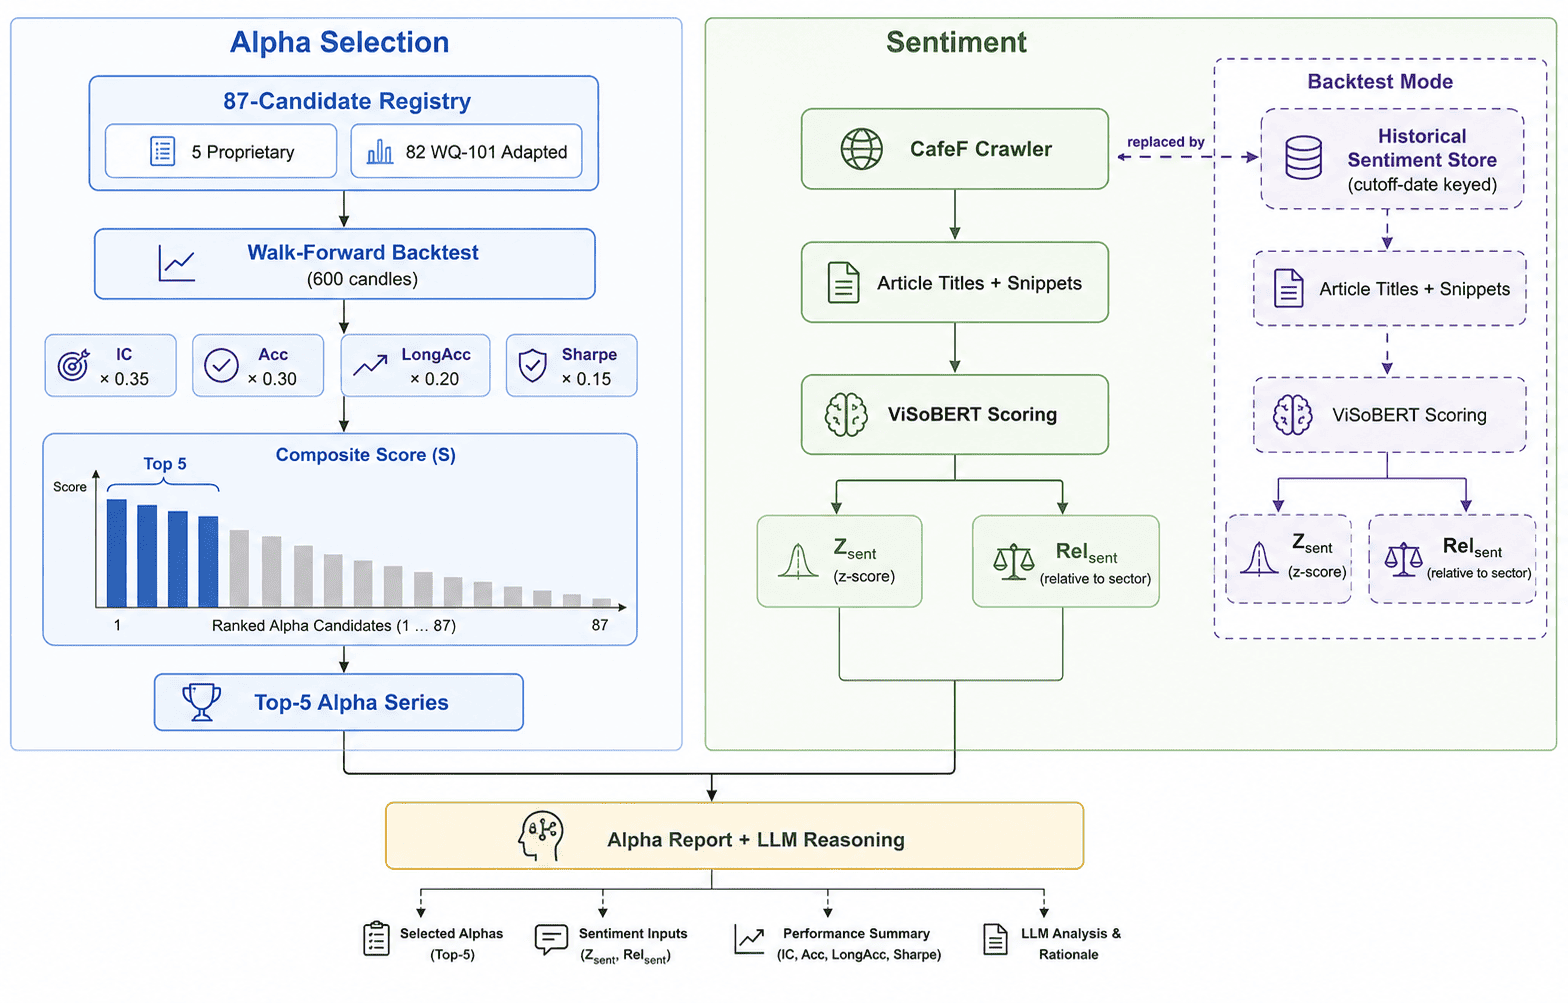
\includegraphics[width=0.9\textwidth]{figs/alpha_agent_pipeline.png}
    \caption{Internal data flow of the Alpha Agent}
    \label{fig:alpha_agent}
\end{figure}

\subsection{Pattern Agent}

The Pattern Agent analyses a candlestick chart rendered from the current
analysis window $[e-W,e)$ (45 candles in the main configuration). The chart is
produced by \texttt{mplfinance} using a custom colour scheme (green bodies for
bearish candles and red bodies for bullish candles, following Vietnamese market
convention) and encoded as a base64 PNG before graph execution.

The vision-language model is prompted to perform four sequential tasks. First, it identifies the dominant chart formation from a curated list of 16 classical patterns, such as head-and-shoulders inverse, double bottom, or various triangles and wedges. Second, it describes the three to five most recent candles in terms of body size, wick length, and relative position. Third, it assesses whether a breakout or breakdown is occurring. Finally, it commits to a directional bias (\texttt{bullish}, \texttt{bearish}, or \texttt{neutral}) alongside a confidence rating of \texttt{High}, \texttt{Medium}, or \texttt{Low}.

The prompt is explicitly structured to discourage non-committal answers and encourage a directional interpretation whenever sufficient evidence is present.

After inference, a deterministic verifier compares the reported bias with the final candlestick body and the direction of the last five closes. An obvious contradiction is appended to the report and downgrades its confidence. If the vision model fails or no chart image is available, the agent falls back to a text-only analysis of raw OHLCV values using the text LLM.


\subsection{Trend Agent}

The Trend Agent receives a separate chart in which support and resistance lines have been fitted algorithmically before LLM invocation.

Two trendline pairs are computed.

\paragraph{Close-price trend channel.}
The first pair is derived from the closing price series alone. A linear regression line is fitted to all 45 candles in $[e-W,e)$, and the upper and lower deviations from this line identify the resistance and support pivots respectively. The slopes are then refined by minimising squared deviations subject to two constraints: the support line must not intersect any closing price from above, and the resistance line must not intersect any closing price from below.

\paragraph{High-low channel.}
The second pair uses the high and low price series to identify the highest and lowest deviation points, producing channel lines that bound the full intra-bar range.

The support lines are drawn in blue, resistance lines in red, and rendered at 600 DPI to preserve legibility when compressed to base64.

The vision-language model is prompted to assess the slope of each support and resistance line, evaluate the distance between the lines (indicating channel width and price compression), determine the position of the most recent candles relative to each boundary, and produce a directional forecast for the applicable prediction horizon. The required JSON output fields encompass the trend direction, numerical support and resistance levels, slope characterisation, and overall confidence.

After inference, a deterministic verifier checks the reported trend against price relative to SMA20, the availability of SMA50, and the recent price slope. Contradictory claims are flagged and their confidence is reduced. If the vision-language model fails or no rendered chart is available, the agent falls back to a text-only analysis of raw OHLCV data, mirroring the strategy used by the Pattern Agent.


\subsection{Decision Agent}

The Decision Agent synthesises all upstream reports into a single trading judgment. To remain within the Groq token-per-minute limit, each report is condensed before being passed to the prompt: the Indicator report is trimmed to its consensus summary block, the Alpha report retains only the factor table and LLM reasoning paragraph, and the Sentiment report drops the per-article listing.

\begin{figure}[htb]
    \centering
    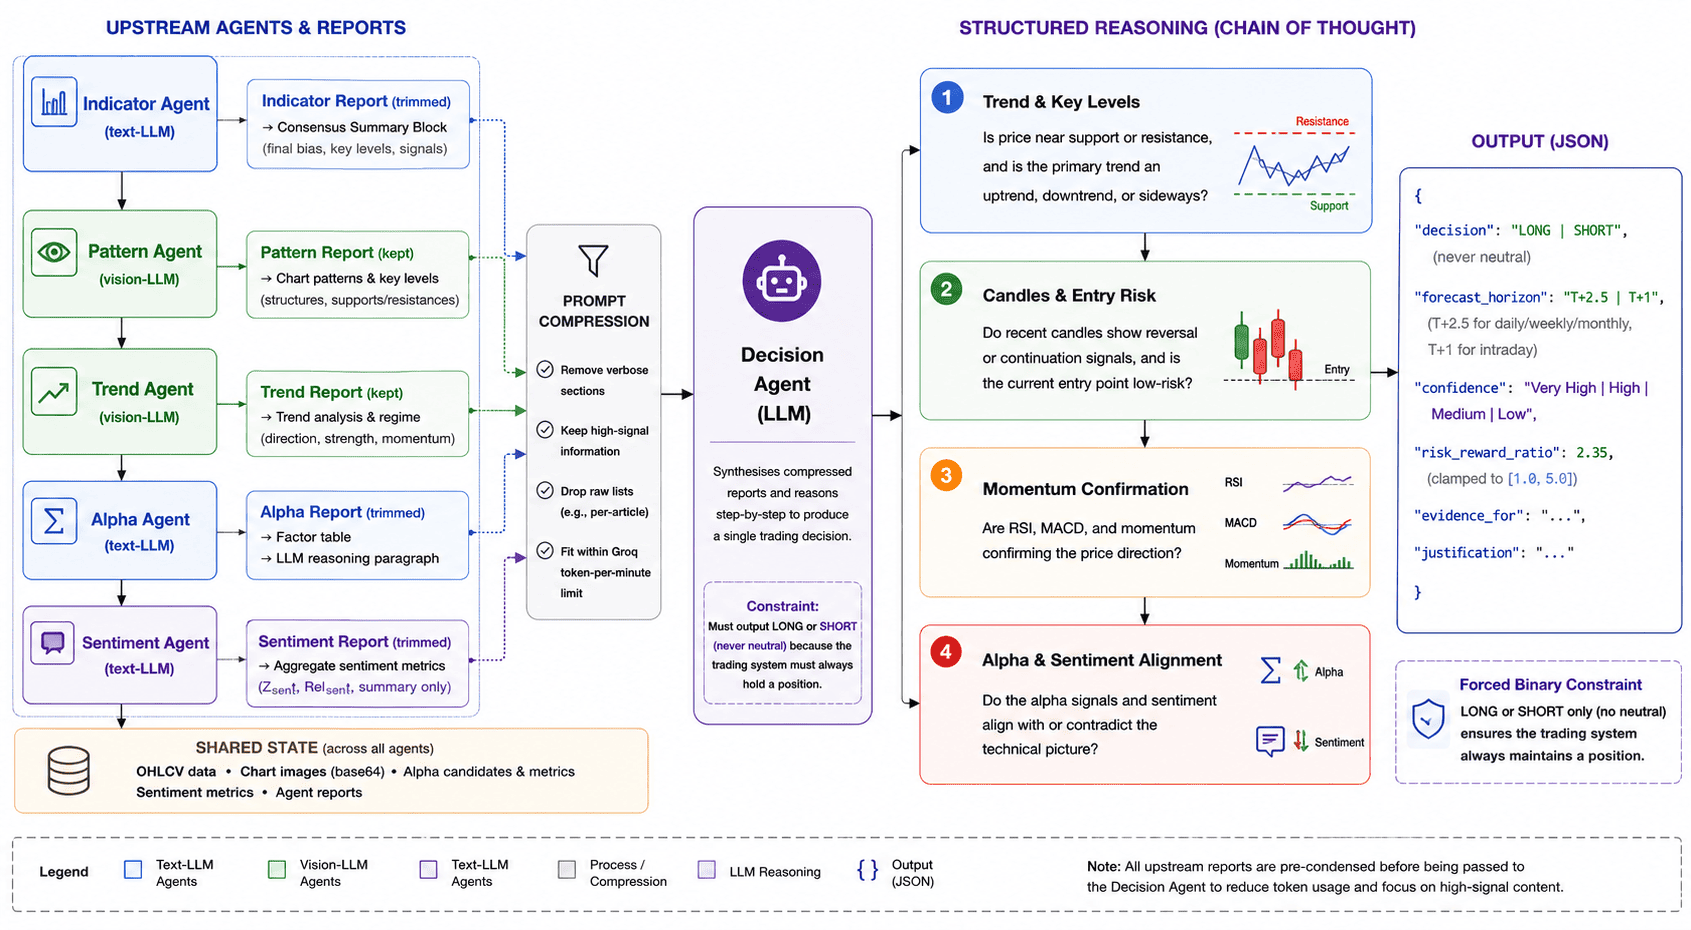
\includegraphics[width=0.95\textwidth]{figs/decision_agent_pipeline.png}
    \caption{Decision Agent reasoning pipeline}
    \label{fig:decision_agent}
\end{figure}

The agent is prompted to reason through four sequential questions in a structured chain-of-thought process. It evaluates whether the price is near support or resistance while identifying the primary trend, checks if recent candles show reversal or continuation signals to ensure a low-risk entry, verifies whether technical oscillators like RSI and MACD confirm the price direction, and finally assesses if the quantitative alpha signals and sentiment align with or contradict the technical picture.

Following this reasoning, the model must output a JSON object comprising a forced binary direction forecast (\texttt{LONG} or \texttt{SHORT}), the \texttt{forecast\_horizon}, the \texttt{confidence} level, a \texttt{risk\_reward\_ratio} clamped to $[1.0, 5.0]$, supporting and opposing evidence, and a final \texttt{justification} paragraph. The prompt explicitly states that this label is not proof of an executed order.

The forced binary constraint supports direction classification only. Downstream account logic independently maps predictions to actions: \texttt{SHORT} maps to \texttt{CASH}, whereas \texttt{LONG} invests all available cash at the next open and closes the position at the configured target close after applying costs on both legs.

\section{Experimental Setup}
\label{sec:experimentalsetup}

\subsection{Dataset and Point-in-Time Data Contract}

The daily evaluation universe contains nine Vietnamese equities spanning technology, aviation, banking, retail, and consumer staples: BHN, CMG, FPT, HVN, MBB, MWG, VCB, VJC, and VNM. The benchmark contains 20 chronologically ordered test points per symbol, for 180 paired observations in total. Section~\ref{sec:limitations_futurework} discusses the limits of this deliberately small universe; the ticker-selection rationale and sentiment-coverage audit are reported separately from the performance analysis.

OHLCV observations are obtained through the project's \texttt{vnstock}-based data loader. At an exclusive test boundary $e$, every agent sees only bars in $[e-W,e)$, so the last visible decision bar is $d=e-1$. Dynamic alpha selection receives a cutoff-safe prefix ending at the same decision bar and containing at most 600 observations. Neither the factor calculations nor the chart renderers can inspect the entry bar or target bar. The numerical, candlestick, and trend inputs use the same requested window length and fail closed when a complete window is unavailable.

The historical sentiment store applies the same cutoff. Only records with a parseable availability date no later than $d$ are eligible; undated records are rejected in research mode instead of being borrowed from a later cache state. The sentiment pathway remains text context for the Decision Agent and does not enter any OHLCV alpha formula.

\subsection{Walk-Forward Protocol}

All reported experiments use daily observations. The main configuration is $W=45$, step size $S=3$, and lookahead $L=3$. For boundary $e$, the simulated entry is the next open $O_e$ and the target exit is $C_{e-1+L}$. The realised net return of a candidate LONG cycle is
\begin{equation}
 r^{\mathrm{net}}_{e,L}
 =\frac{C_{e-1+L}}{O_e}
  \frac{(1-c_{\mathrm{slip}})(1-c_{\mathrm{fee}})}
       {(1+c_{\mathrm{slip}})(1+c_{\mathrm{fee}})}-1,
 \label{eq:execution_return_setup}
\end{equation}
where $c_{\mathrm{fee}}=0.0025$ and $c_{\mathrm{slip}}=0.001$ are applied separately on both the BUY and SELL legs. The economic direction label is \texttt{UP} only when $r^{\mathrm{net}}_{e,L}>0$ and is \texttt{DOWN} otherwise. This definition makes the classification target, alpha-selection target, and account return share the same Open-to-Close horizon and cost convention.

\begin{table}[H]
\centering
\caption{Main walk-forward configuration.}
\label{tab:backtest_hyperparameters}
\renewcommand{\arraystretch}{1.18}
\begin{tabularx}{\textwidth}{|l|l|X|}
\hline
\textbf{Parameter} & \textbf{Value} & \textbf{Operational meaning} \\
\hline
Analysis window $W$ & 45 bars & Exact agent input $[e-W,e)$ \\
\hline
Step size $S$ & 3 bars & Separation between consecutive test boundaries \\
\hline
Lookahead $L$ & 3 bars & Entry at $O_e$ and exit at $C_{e-1+L}$ \\
\hline
Test points & 20 per symbol & 180 paired observations over nine symbols \\
\hline
Alpha history & Up to 600 bars & Cutoff-safe calibration/evaluation prefix ending at $d=e-1$ \\
\hline
Alpha registry & 85 candidates & Top five selected at each test point \\
\hline
Random seeds & 42 & Python/NumPy and bootstrap reproducibility \\
\hline
\end{tabularx}
\end{table}

\subsection{Paired Baseline and Disentangled Ablations}

The primary benchmark compares the Full System with a No-Alpha baseline under the implemented \texttt{paired\_shared\_reports} protocol. Indicator, Pattern, and Trend agents run once at each cutoff. Their immutable report snapshot is deep-copied into both decision branches, so only the Alpha bundle and the corresponding final decision differ. This eliminates upstream LLM and chart-generation variation within each pair. All 180 benchmark pairs produced valid binary decisions.

\begin{table}[H]
\centering
\caption{Paired benchmark variants.}
\label{tab:system_variants}
\renewcommand{\arraystretch}{1.2}
\begin{tabularx}{\textwidth}{|l|X|X|}
\hline
\textbf{Component} & \textbf{Full System} & \textbf{No-Alpha baseline} \\
\hline
Indicator report & Shared upstream snapshot & Identical shared snapshot \\
\hline
Pattern and Trend reports & Shared upstream snapshot & Identical shared snapshot \\
\hline
OHLCV alpha factors & Enabled & Disabled \\
\hline
Vietnamese sentiment context & Enabled & Disabled \\
\hline
Final Decision Agent & Receives all enabled reports & Receives only shared upstream reports \\
\hline
\end{tabularx}
\end{table}

To separate the two components bundled in the primary intervention, a second experiment uses the \texttt{four\_way\_shared\_upstream} protocol on FPT, VNM, and VCB. It evaluates Full (factors and sentiment), Alpha-only (factors), Sentiment-only (sentiment), and Baseline (neither). All four branches receive the same upstream snapshot at each test point. The independent directional contributions are defined relative to Baseline, while the interaction is
\begin{equation}
 \mathrm{Synergy}
 =\mathrm{Acc}_{\mathrm{Full}}
 -\max\!\left(\mathrm{Acc}_{\mathrm{AlphaOnly}},
               \mathrm{Acc}_{\mathrm{SentimentOnly}}\right).
 \label{eq:ablation_synergy}
\end{equation}

\clearpage
\subsection{Account and Statistical Metrics}

Each variant starts with VND~50,000,000 and is simulated independently. Every LONG uses all available cash at $O_e$, pays fee and slippage on purchase, sells all shares at $C_{e-1+L}$, and pays both costs again on sale. Every cycle therefore ends in cash before the next test point. A SHORT forecast is a directional prediction only and maps to CASH because uncovered short selling of the underlying equity is disabled. With cycle return $q_k=r^{\mathrm{net}}_{e_k,L}$ for LONG and $q_k=0$ for SHORT, wealth compounds as
\begin{equation}
 W_{k+1}=W_k(1+q_k),\qquad
 R_{\mathrm{acct}}=\frac{W_K}{W_0}-1.
 \label{eq:account_return_setup}
\end{equation}

Account Sharpe is the mean of the 20 cycle returns divided by their population standard deviation and annualised by $\sqrt{252}$; CASH cycles contribute zero. Maximum drawdown is computed from the compounded cycle-end equity curve anchored at $W_0$. These metrics describe the stated research simulation rather than a deployable execution strategy: spread variation, partial fills, taxes, liquidity limits, and market impact are outside the model.

Statistical inference is computed on paired common support. For each symbol, an exact two-sided McNemar test compares discordant correctness outcomes. A moving-block bootstrap with block length five, 1,000 replications, and seed 42 yields the 95\% interval for Alpha Lift. A Newey--West test is also stored for the paired correctness-difference series. Across the nine symbols, a two-sided Wilcoxon signed-rank test evaluates whether the symbol-level lifts are centred at zero.

\begin{table}[H]
\centering
\caption{Evaluation metrics and estimands.}
\label{tab:evaluation_metrics}
\renewcommand{\arraystretch}{1.16}
\begin{tabularx}{\textwidth}{|l|X|}
\hline
\textbf{Metric} & \textbf{Definition} \\
\hline
Directional accuracy & Fraction of valid LONG/SHORT forecasts matching the net economic direction in Eq.~\eqref{eq:label}. \\
\hline
Alpha Lift & Full accuracy minus the accuracy of its paired No-Alpha branch, in percentage points. \\
\hline
Account return & Compounded fixed-cycle return $W_K/W_0-1$; LONG executes and SHORT holds cash. \\
\hline
Account Sharpe & Mean cycle return divided by population standard deviation and annualised by $\sqrt{252}$. \\
\hline
Maximum drawdown & Largest peak-to-trough decline on the compounded cycle-end equity curve. \\
\hline
Paired inference & Exact McNemar test, moving-block 95\% lift interval, Newey--West mean test, and cross-symbol Wilcoxon signed-rank test. \\
\hline
\end{tabularx}
\end{table}

\subsection{Implementation and Robustness Design}

The text model is \texttt{openai/gpt-oss-20b} and the vision model is \texttt{qwen/qwen3.8-27b}; both use temperature zero in the reported runs. Hosted inference can nevertheless remain nondeterministic. Calls are executed sequentially with rate-limit pacing, and checkpoint files permit completed test points to be resumed without changing their stored outputs.

\begin{table}[H]
\centering
\caption{Implementation configuration used by the reported experiments.}
\label{tab:implementation_details}
\renewcommand{\arraystretch}{1.16}
\begin{tabularx}{\textwidth}{|l|X|}
\hline
\textbf{Component} & \textbf{Configuration} \\
\hline
Text / vision models & \texttt{openai/gpt-oss-20b} / \texttt{qwen/qwen3.8-27b}; temperature $0.0$ \\
\hline
Initial capital & VND~50,000,000 independently for each variant \\
\hline
Costs & 0.25\% fee and 0.10\% slippage on each BUY and SELL leg \\
\hline
Position rule & LONG invests all cash for one fixed cycle; SHORT remains in CASH \\
\hline
Primary protocol & \texttt{paired\_shared\_reports}; 20 test points per symbol \\
\hline
Four-way protocol & \texttt{four\_way\_shared\_upstream}; Full, Alpha-only, Sentiment-only, Baseline \\
\hline
\end{tabularx}
\end{table}

The robustness experiment evaluates FPT and VNM with 20 test points per configuration. Panel A changes the common analysis window to $W\in\{30,45,60\}$. Panel B compares \texttt{zscore\_tanh}, \texttt{minmax}, and \texttt{rank} alpha normalisation. Panel C compares default, equal, and IC-heavy ranking weights. For Panels B and C, the No-Alpha branch is reused from the same shared upstream/control checkpoint within each symbol and panel; its decisions must therefore be invariant to parameters that only affect the Alpha branch. Panel A deliberately changes the shared input window, so its No-Alpha output is not expected to remain constant across rows.

\section{Backtest Results}
\label{sec:backtestresults}

\subsection{Nine-Symbol Paired Benchmark}

Table~\ref{tab:overall_results} reports the completed paired benchmark. The Full System attains mean directional accuracy of 65.0\%, compared with 51.1\% for No-Alpha, for a mean Alpha Lift of +13.9 percentage points (pp). Eight symbols have positive lift and VJC has zero lift. The cross-symbol Wilcoxon signed-rank test rejects a zero-centred lift ($p=0.0078$), although none of the individual exact McNemar tests reaches the 5\% level with only 20 paired points per symbol. The moving-block intervals are correspondingly wide; VCB is the only symbol whose reported 95\% lift interval excludes zero.

\begin{table}[!htb]
\centering
\caption{Paired benchmark over nine equities ($N=20$ per symbol, $W=45$, $S=3$, $L=3$). Panel A reports directional inference; Panel B reports compounded long-only account outcomes.}
\label{tab:overall_results}
\renewcommand{\arraystretch}{1.12}
\setlength{\tabcolsep}{3.2pt}

\textit{Panel A: Directional accuracy and paired inference}

\resizebox{\columnwidth}{!}{%
\begin{tabular}{lrrrrrr}
\hline
\textbf{Symbol} & \textbf{Full (\%)} & \textbf{No-$\alpha$ (\%)} & \textbf{Lift (pp)} & \textbf{95\% CI (pp)} & \textbf{McNemar $p$} & \textbf{$N$} \\
\hline
BHN & 55.0 & 45.0 & +10.0 & $[+0.0,+15.0]$ & 0.6875 & 20 \\
CMG & 75.0 & 70.0 & +5.0 & $[+0.0,+5.0]$ & 1.0000 & 20 \\
FPT & 65.0 & 45.0 & +20.0 & $[-5.0,+35.0]$ & 0.2188 & 20 \\
HVN & 70.0 & 50.0 & +20.0 & $[+0.0,+35.0]$ & 0.2188 & 20 \\
MBB & 70.0 & 45.0 & +25.0 & $[+0.0,+55.0]$ & 0.1250 & 20 \\
MWG & 70.0 & 50.0 & +20.0 & $[+0.0,+40.0]$ & 0.1250 & 20 \\
VCB & 65.0 & 50.0 & +15.0 & $[+5.0,+35.0]$ & 0.2500 & 20 \\
VJC & 60.0 & 60.0 & +0.0 & $[-10.0,+10.0]$ & 1.0000 & 20 \\
VNM & 55.0 & 45.0 & +10.0 & $[-15.0,+45.0]$ & 0.6250 & 20 \\
\hline
\textbf{Mean} & \textbf{65.0} & \textbf{51.1} & \textbf{+13.9} & -- & -- & \textbf{20} \\
\hline
\end{tabular}}

\vspace{0.7em}
\textit{Panel B: Compounded account metrics}

\resizebox{\columnwidth}{!}{%
\begin{tabular}{lrrrrrr}
\hline
\textbf{Symbol} & \textbf{Return F (\%)} & \textbf{Return N (\%)} & \textbf{Sharpe F} & \textbf{Sharpe N} & \textbf{MDD F (\%)} & \textbf{MDD N (\%)} \\
\hline
BHN & -4.20 & -5.76 & -3.63 & -2.64 & 4.80 & 8.31 \\
CMG & -2.66 & -5.60 & -3.64 & -5.28 & 2.66 & 5.60 \\
FPT & -1.56 & -10.37 & -0.86 & -6.41 & 6.30 & 10.37 \\
HVN & +2.89 & -15.64 & +1.19 & -4.27 & 5.27 & 20.06 \\
MBB & +5.21 & -7.78 & +2.36 & -4.22 & 3.50 & 9.89 \\
MWG & +0.39 & -6.42 & +0.41 & -3.93 & 1.92 & 8.17 \\
VCB & -8.34 & -10.49 & -5.98 & -7.78 & 8.92 & 10.49 \\
VJC & -6.05 & -6.26 & -5.22 & -5.38 & 6.05 & 6.26 \\
VNM & -0.85 & -7.51 & -0.41 & -4.91 & 3.40 & 7.51 \\
\hline
\textbf{Mean} & \textbf{-1.69} & \textbf{-8.43} & \textbf{-1.75} & \textbf{-4.98} & \textbf{4.76} & \textbf{9.63} \\
\hline
\end{tabular}}

\vspace{0.4em}
\begin{flushleft}\footnotesize
F and N denote Full and No-Alpha. The 95\% intervals use a moving-block bootstrap (block length 5; 1,000 replications). The two-sided cross-symbol Wilcoxon result is $p=0.0078125$ (nine symbol-level lifts; median lift $=15.0$ pp). Returns are compounded from VND~50,000,000 independent accounts under Eq.~\eqref{eq:account_return}; SHORT forecasts remain in cash.
\end{flushleft}
\end{table}

The economic results are materially more cautious than the directional results. Full outperforms No-Alpha in account return for all nine symbols, but its mean account return is still $-1.69\%$, and only HVN, MBB, and MWG finish positive. Hence the experiment supports a paired directional improvement and a relative reduction in losses, not general profitability. The divergence is expected under the long-only action map: a correct SHORT improves directional accuracy but earns a zero account return.

\subsection{Robustness and Sensitivity}

Table~\ref{tab:robustness_results} reports all six completed sweeps. Each row contains 20 paired test points. Panel A changes the input window for both variants and therefore changes the No-Alpha information set. In Panels B and C, which intervene only on Alpha processing, the No-Alpha accuracy is exactly invariant within each symbol and panel: 45.0\% for both normalisation sweeps, 50.0\% for the FPT weight sweep, and 45.0\% for the VNM weight sweep.

\begin{table}[!htb]
\centering
\caption{Robustness sweep on FPT and VNM ($N=20$ per row). Returns are compounded account returns.}
\label{tab:robustness_results}
\renewcommand{\arraystretch}{1.08}
\setlength{\tabcolsep}{2.8pt}
\resizebox{\columnwidth}{!}{%
\begin{tabular}{lllrrrrr}
\hline
\textbf{Symbol} & \textbf{Panel} & \textbf{Scenario} & \textbf{Full (\%)} & \textbf{No-$\alpha$ (\%)} & \textbf{Lift (pp)} & \textbf{Return F (\%)} & \textbf{Return N (\%)} \\
\hline
FPT & Window & $W=30$ & 55.0 & 40.0 & +15.0 & -2.63 & -10.27 \\
FPT & Window & $W=45$ & 65.0 & 50.0 & +15.0 & -2.21 & -6.86 \\
FPT & Window & $W=60$ & 40.0 & 45.0 & -5.0 & -8.04 & -4.38 \\
VNM & Window & $W=30$ & 40.0 & 40.0 & +0.0 & -7.81 & -7.51 \\
VNM & Window & $W=45$ & 55.0 & 40.0 & +15.0 & -3.59 & -7.06 \\
VNM & Window & $W=60$ & 65.0 & 55.0 & +10.0 & +5.20 & -0.84 \\
\hline
FPT & Normalisation & \texttt{zscore\_tanh} & 50.0 & 45.0 & +5.0 & -4.72 & -7.38 \\
FPT & Normalisation & \texttt{minmax} & 55.0 & 45.0 & +10.0 & -5.63 & -7.38 \\
FPT & Normalisation & \texttt{rank} & 60.0 & 45.0 & +15.0 & -4.36 & -7.38 \\
VNM & Normalisation & \texttt{zscore\_tanh} & 60.0 & 45.0 & +15.0 & +2.70 & -2.22 \\
VNM & Normalisation & \texttt{minmax} & 65.0 & 45.0 & +20.0 & +3.89 & -2.22 \\
VNM & Normalisation & \texttt{rank} & 55.0 & 45.0 & +10.0 & -2.01 & -2.22 \\
\hline
FPT & Weighting & \texttt{default} & 60.0 & 50.0 & +10.0 & -1.99 & -7.85 \\
FPT & Weighting & \texttt{equal\_weight} & 60.0 & 50.0 & +10.0 & -0.36 & -7.85 \\
FPT & Weighting & \texttt{ic\_heavy} & 65.0 & 50.0 & +15.0 & -2.21 & -7.85 \\
VNM & Weighting & \texttt{default} & 65.0 & 45.0 & +20.0 & +6.17 & -5.19 \\
VNM & Weighting & \texttt{equal\_weight} & 50.0 & 45.0 & +5.0 & -4.57 & -5.19 \\
VNM & Weighting & \texttt{ic\_heavy} & 60.0 & 45.0 & +15.0 & +2.70 & -5.19 \\
\hline
\end{tabular}}
\end{table}

The alpha-enabled branch is sensitive to configuration. In particular, FPT at $W=60$ produces a $-5.0$ pp lift, and VNM at $W=30$ produces no lift. The normalisation and weighting panels remain positive for both symbols, but their Full accuracies and economic returns vary materially. These results validate the paired-control implementation while also showing that the intervention is not uniformly robust to window choice or alpha design.

\subsection{Disentangled Alpha--Sentiment Ablation}

Table~\ref{tab:disentangled_ablation} separates quantitative factors from Vietnamese sentiment context on three representative symbols. Alpha-only improves directional accuracy for every symbol, with a mean independent contribution of +8.33 pp. Sentiment-only contributes +5.0 pp for VNM and 0.0 pp for FPT and VCB, giving a mean independent contribution of +1.67 pp. The interaction is heterogeneous: +5.0 pp for FPT, +10.0 pp for VNM, and $-10.0$ pp for VCB.

\begin{table}[!htb]
\centering
\caption{Four-way shared-upstream ablation ($N=20$ per variant and symbol).}
\label{tab:disentangled_ablation}
\renewcommand{\arraystretch}{1.1}
\setlength{\tabcolsep}{3pt}

\textit{Panel A: Directional decomposition}

\resizebox{\columnwidth}{!}{%
\begin{tabular}{lrrrrrrr}
\hline
\textbf{Symbol} & \textbf{Full} & \textbf{Alpha-only} & \textbf{Sent.-only} & \textbf{Baseline} & \textbf{$\Delta\alpha$} & \textbf{$\Delta$Sent.} & \textbf{Synergy} \\
\hline
FPT & 55.0\% & 50.0\% & 45.0\% & 45.0\% & +5.0 pp & +0.0 pp & +5.0 pp \\
VNM & 60.0\% & 50.0\% & 50.0\% & 45.0\% & +5.0 pp & +5.0 pp & +10.0 pp \\
VCB & 45.0\% & 55.0\% & 40.0\% & 40.0\% & +15.0 pp & +0.0 pp & -10.0 pp \\
\hline
\textbf{Mean} & \textbf{53.33\%} & \textbf{51.67\%} & \textbf{45.00\%} & \textbf{43.33\%} & \textbf{+8.33 pp} & \textbf{+1.67 pp} & \textbf{+1.67 pp} \\
\hline
\end{tabular}}

\vspace{0.7em}
\textit{Panel B: Compounded account return}

\begin{tabular}{lrrrr}
\hline
\textbf{Symbol} & \textbf{Full} & \textbf{Alpha-only} & \textbf{Sentiment-only} & \textbf{Baseline} \\
\hline
FPT & -4.61\% & -7.85\% & -7.38\% & -6.09\% \\
VNM & -4.03\% & +2.26\% & -5.86\% & -3.96\% \\
VCB & -7.93\% & -2.75\% & -9.23\% & -11.34\% \\
\hline
\end{tabular}
\end{table}

The ablation does not support attributing the entire primary benchmark lift to sentiment. The factor pathway provides the more consistent independent directional increment, whereas sentiment is useful only for VNM in this sample. VCB also demonstrates negative interaction: combining sentiment with factors reduces accuracy relative to Alpha-only by 10.0 pp. Economic ordering differs again from directional ordering; for example, VNM Alpha-only is profitable (+2.26\%) while its Full variant loses 4.03\%. These findings motivate larger-sample interaction tests rather than a universal claim that additional modalities always improve decisions.

\section{Limitations \& Future Work}
\label{sec:limitations_futurework}

\subsection{Limitations}

\paragraph{L1. Statistical scale and economic interpretation.}
The paired benchmark controls upstream reports and evaluates 180 decisions, but each symbol contributes only 20 observations. Moving-block confidence intervals and exact McNemar tests correctly expose this low per-symbol power: no individual McNemar result is significant at 5\%, even though the cross-symbol Wilcoxon test is significant. The nine tickers are also not a probability sample of the Vietnamese market. Results should therefore be read as evidence for this benchmark universe rather than a market-wide performance estimate.

Directional skill and economic value remain distinct. The Full System raises mean accuracy by 13.9 pp and improves account return relative to No-Alpha for every symbol, yet its mean compounded return is $-1.69\%$ and only three symbols finish positive. Correct SHORT forecasts earn no return because the cash-equity simulator maps SHORT to CASH. Consequently, the reported lift does not establish deployable profitability.

\paragraph{L2. Simplified execution model.}
The fixed-cycle ledger removes the previous horizon mismatch: labels, alpha targets, and account returns all use the same next-open-to-target-close net return, wealth is compounded, and fee plus slippage are charged on both BUY and SELL. Nevertheless, the constants are benchmark assumptions. The model omits time-varying bid--ask spreads, taxes, order-book depth, partial fills, volume-dependent market impact, position limits, and portfolio competition among simultaneous symbols. It also assumes that each $S=L=3$ cycle is closed before the next entry. A venue-calibrated event-driven simulator is required before live deployment.

\paragraph{L3. Alpha selection and sensitivity.}
Selecting five factors from an 85-candidate registry creates multiple-testing and selection risks. The point-in-time cutoff prevents future leakage, and the composite score uses $0.40|\mathrm{IC}|+0.35\mathrm{Accuracy}+0.25\mathrm{Sharpe}$, but short calibration histories can still make signal orientation and ranking unstable. The robustness results confirm this concern: FPT produces a negative lift at $W=60$, and performance changes materially across normalisation and weighting schemes. Furthermore, translating cross-sectional WorldQuant operators into single-asset time-series operators changes their economic and statistical meaning.

\paragraph{L4. Hosted-model and visual reliability.}
Temperature zero and fixed prompts do not guarantee bitwise deterministic output from hosted models. The paired design removes upstream variation within a Full/No-Alpha comparison, but separate runs can still differ because of provider-side model updates or inference nondeterminism. Pattern and Trend agents now compare visual conclusions with deterministic OHLCV rules and downgrade contradictory outputs; this gate reduces obvious chart hallucinations but is not a substitute for an externally labelled pattern-recognition benchmark.

\paragraph{L5. Sentiment coverage and attribution.}
Strict cutoff filtering prevents future and undated articles from entering a historical decision. Coverage can nevertheless be sparse and uneven across firms, particularly for smaller or less news-intensive equities. The three-symbol ablation finds a positive independent sentiment contribution only for VNM and a negative factor--sentiment interaction for VCB. This heterogeneity limits any broad causal claim about Vietnamese news sentiment.

\subsection{Future Work}

\paragraph{F1. Larger and longer evaluation.}
The most important extension is a preregistered study over a broader universe such as the VN100 and multiple market regimes. More test points would increase per-symbol power, support sector-level analysis, and permit out-of-time validation rather than repeated analysis of the same recent period.

\paragraph{F2. Stronger baselines and multiplicity control.}
Future experiments should add random-walk, logistic, tree-based, and sequence-model baselines on the identical information set. White's Reality Check, false-discovery-rate control, or the Deflated Sharpe Ratio should accompany factor selection to account for searching across 85 candidates.

\paragraph{F3. Execution and portfolio realism.}
A portfolio simulator should model lot sizes, taxes, dynamic spreads, liquidity limits, partial fills, and market impact, and should allocate capital jointly across symbols. Confidence gates and risk-based sizing can then be assessed without conflating forecasting accuracy with all-in binary allocation.

\paragraph{F4. Component reliability.}
Repeated hosted-model runs should quantify decision variance. Vision outputs should be compared with deterministic pattern detectors and human-labelled charts, while sentiment should be evaluated against a Vietnamese financial-domain test set. The observed negative VCB interaction also motivates an explicit conflict-resolution mechanism between factor and sentiment evidence.

\subsection{Broader Impact}

Localized financial AI can broaden research beyond English-language, highly liquid markets, but automated use in a shallow market may amplify noise and herding. The framework should therefore be treated as decision-support research rather than trading advice. Reproducible releases must preserve model and data provenance while respecting news copyright, provider terms, and privacy obligations.

\section{Conclusion}
\label{sec:conclusion}

This study implemented and evaluated a LangGraph multi-agent system for price-driven directional forecasting in Vietnamese equities. Its principal methodological contributions are a point-in-time 85-factor alpha registry, cutoff-safe Vietnamese sentiment context, shared upstream reports for paired comparison, deterministic consistency checks for vision-agent outputs, and a long-only compounded account ledger whose prediction and execution horizons are aligned.

Across nine symbols and 180 paired test points, the Full System achieved mean accuracy of 65.0\%, compared with 51.1\% for No-Alpha, yielding a mean lift of +13.9 pp. Eight symbols improved and one tied; the cross-symbol Wilcoxon test gave $p=0.0078$. The economic evidence is weaker: Full account return exceeded No-Alpha for every symbol, but the mean Full return remained negative at $-1.69\%$, and only HVN, MBB, and MWG were profitable under the stated cost model. These results support improved relative directional performance, not a claim of general trading profitability.

The robustness study confirms that the No-Alpha control is invariant when only alpha normalisation or weighting changes. It also reveals genuine sensitivity: the Full branch ranges from negative to positive lift across window choices. The four-way ablation further shows that OHLCV alpha factors provide the more consistent independent contribution (+8.33 pp on average across FPT, VNM, and VCB), whereas sentiment contributes +1.67 pp on average and interacts negatively with factors for VCB. Thus multimodal evidence should be gated and validated rather than assumed to be additive. Point-in-time selection removes future-bar leakage but does not remove multiplicity or same-window orientation bias; likewise, deterministic visual consistency checks do not establish that a vision model used the claimed local chart evidence. The 80 WorldQuant-derived candidates remain heuristic single-asset translations whose decay, autocorrelation, and turnover require a dedicated audit.

Overall, the experiments demonstrate the value of leakage-safe, paired evaluation for LLM-based financial agents while exposing the gap between directional accuracy and investable returns. Larger universes, longer out-of-time samples, classical baselines, multiplicity-aware factor selection, repeated hosted-model runs, and venue-calibrated execution remain necessary before practical deployment.


%% CRediT authorship contribution statement
%% (elsarticle.cls has no \credit/\printcredits macros; the CRediT
%% roles from the original cas-sc source are preserved here verbatim
%% as a standard Elsevier "CRediT authorship contribution statement"
%% section instead.)
\section*{CRediT authorship contribution statement}

\textbf{Van-Tang Nguyen:} Conceptualization (C); Software (So); Validation (Va); Investigation (I); Original draft preparation (O); Project administration (P); Funding acquisition (Fu).

\textbf{Hoang-Dung Phan:} Methodology (M); Software (So); Formal analysis (Fo); Investigation (I); Resources (R); Data curation (D); Original draft preparation (O); Writing-review and editing (E); Visualization (Vi); Supervision (Su).

\textbf{Thanh-Tam Do Thi:} Methodology (M); Investigation (I); Data curation (D); Original draft preparation (O); Writing-review and editing (E); Supervision (Su).

\textbf{Phuong-Thai Nguyen:} Methodology (M); Investigation (I); Data curation (D); Original draft preparation (O); Visualization (Vi); Supervision (Su).

\textbf{Hong-Viet Tran:} Conceptualization (C); Methodology (M); Software (So); Validation (Va); Formal analysis (Fo); Data curation (D); Original draft preparation (O); Writing-review and editing (E); Project administration (P).

\section*{CONFLICT OF INTEREST STATEMENT (mandatory)}
Authors state no conflict of interest.

% \section*{INFORMED CONSENT (if applicable)}
% The protection of privacy is a legal right that must not be breached without individual informed consent. In cases where the identification of personal information is necessary for scientific reasons, authors should obtain full documentation of informed consent, including written permission from the patient prior to inclusion in the study. Incorporate the following (or a similar) statement: We have obtained informed consent from all individuals included in this study.

% \section*{ETHICAL APPROVAL (if applicable)}
% When papers talk about using people or animals, authors should make it clear that the research followed all national rules and institutional policies, and it was approved by the authors' institutional review board or a similar committee. The Helsinki Declaration's tenets must guide all investigations involving human subjects. Authors must also identify the committee or review board approving the experiments and provide a statement indicating approval of the research. Incorporate the following (or a similar) statement: The research related to human use has been complied with all the relevant national regulations and institutional policies in accordance with the tenets of the Helsinki Declaration and has been approved by the authors' institutional review board or equivalent committee; or: The research related to animal use has been complied with all the relevant national regulations and institutional policies for the care and use of animals.

\section*{DATA AVAILABILITY (mandatory)}
\begin{itemize}[topsep=0.3ex, itemsep=0.3ex, parsep=0.2ex]
    \item[-]The supporting data of this study are openly available from the CafeF at https://cafef.vn~ financial information platform and consist of publicly accessible financial reports of Vietnamese enterprises.

    % \item[-] The data that support the findings of this study are available on request from the corresponding author, [initials: AB]. The data, which contain information that could compromise the privacy of research participants, are not publicly available due to certain restrictions.
    % \item[-] Derived data supporting the findings of this study are available from the corresponding author [initials: AB] on request.
    % \item[-] The data that support the findings of this study are available from [third party]. Restrictions apply to the availability of these data, which were used under license for this study. Data are available [from the authors / at URL] with the permission of [third party].
% \item[-] The authors confirm that the data supporting the findings of this study are available within the article [and/or its supplementary materials].
    % \item[-] The data that support the findings of this study are available from the corresponding author, [initials: AB], upon reasonable request.
    % \item[-] Data availability is not applicable to this paper as no new data were created or analyzed in this study.
\end{itemize}
\section*{CODE AVAILABILITY}
\begin{itemize}[topsep=0.3ex, itemsep=0.3ex, parsep=0.2ex]
    \item[-]A demonstration chatbot system developed from the proposed framework is available in the \href{https://github.com/DungPhanHoangg05/A-Multi-Agent-Large-Language-Model-Approach-to-Price-Driven-Stock-Trading-in-the-Vietnamese-Stock-Ma.git}{project repository}.

\end{itemize}

\section*{Acknowledgments}
This research is funded by Foreign Trade University under research program number FTURP02-2026-08


%% ── APPENDIX ──────────────────────────────────────────────────────────────────


\appendix

\section{Agent System Prompts}
\label{app:prompts}

This appendix presents the system and user prompts deployed in the agents.

\textit{Note: The original prompts in the codebase are written entirely in Vietnamese to match the target market's language conventions and to elicit native-level analysis from the LLMs. For the purpose of this paper, they have been translated into English and condensed, while strictly preserving their original logic, constraints, and instructions.}

\subsection{Decision Agent Prompt}
\label{app:prompt_decision}

The Decision Agent receives all upstream reports condensed to save tokens. The prompt enforces a forced binary direction forecast (LONG or SHORT), explicitly distinct from an executed action, and a structured reasoning process. The forecast horizon is dynamically injected as a bar count (e.g., \texttt{L=3 bars} for daily data), never as settlement notation. Below is the prompt template (with placeholder variables denoted by \texttt{\{...\}}):

\begin{framed}
\begin{small}
\begin{verbatim}
You are a Senior Quant Trader with 20 years of experience in the VN stock market.
Asset: **{stock_name}** | Timeframe: **{time_frame}**.

MARKET RULE: {h_note}

TIME-INDEX CONTRACT: the input window is [e-W,e); the final visible decision
bar is d=e-1; candidate entry is at the next-bar open O[e]; the immutable
entry is O[e] and the target exit is C[e-1+L]. The label is UP only
when this LONG cycle remains profitable after costs on both legs.

CORE OBJECTIVE: Deeply evaluate reports from independent AI Agents
to forecast **{h_desc}**. You MUST make a definitive decision:
choose either **LONG** or **SHORT** (NEUTRAL is STRICTLY FORBIDDEN).

---
### [1] TREND ANALYSIS (Trend Agent)
{trend_report}
---
### [2] PRICE PATTERNS (Pattern Agent)
{pattern_report}
---
### [3] TECHNICAL INDICATORS (Indicator Agent)
{indicator_report}
---
### [4] ALPHA FACTORS & ORDER FLOW (Alpha Agent)
{alpha_report}
### [5] NEWS & MARKET SENTIMENT (Sentiment Analysis)
{sentiment_report}
---
## REASONING GUIDE (Chain of Thought)
1. Market Context (Trend)
2. Price Action & Timing (Pattern)
3. Momentum (Indicator)
4. Flow & Sentiment (Alpha + Sentiment)

## MANDATORY OUTPUT FORMAT
```json
{
  "decision": "<LONG or SHORT>",
  "forecast_horizon": "{h_val}",
  "confidence": "<Very High | High | Medium | Low>",
  "risk_reward_ratio": <float>,
  "evidence_for": "<3 sentences summarizing reasons>",
  "evidence_against": "<Biggest risk>",
  "justification": "<Brief justification>"
}
```
\end{verbatim}
\end{small}
\end{framed}

The agent reports 4 (when Alpha Agent is active) or 3 (No-Alpha ablation) upstream summaries. Sections \texttt{[4]} and \texttt{[5]} are omitted entirely when \texttt{include\_alpha=False}.

\subsection{Pattern Agent Prompt}
\label{app:prompt_pattern}

The frozen configuration names the vision-language model \texttt{qwen/qwen3.8-27b}; the following Pattern Agent prompt is prototype source, not a provenance-validated research artifact:

\begin{framed}
\begin{small}
\begin{verbatim}
/no_think
You are an AI specializing in Price Action pattern analysis.

ABSOLUTE RULES:
1. ONLY return the 6 fields below. Do NOT add any other fields.
2. NO reasoning, NO explanations.
3. NO fallback scenarios. Provide exactly ONE definitive assessment.
4. Each field on ONE line. Be concise.

MANDATORY FORMAT:
**Pattern:** <Name>
**Confidence:** High | Medium | Low
**Forecast Bias:** Bullish | Bearish | Neutral
**Evidence:** <Brief description>
**Key Candle:** <List key candle>
**Trade Implication:** <Scenario>
\end{verbatim}
\end{small}
\end{framed}

The 16 reference patterns provided to the model include: Inverse Head and Shoulders, Double Bottom, Falling/Rising Wedge, Triangle, Bull/Bear Flag, Rectangle, V-Reversal, and Clear Trend.

If the vision model fails, the agent falls back to a text-only analysis of the most recent 20 OHLCV rows using the text LLM (\texttt{openai/gpt-oss-20b}).

\subsection{Trend Agent Prompt}
\label{app:prompt_trend}

The Trend Agent also utilizes a vision-language model to evaluate dynamically generated support and resistance lines.

\begin{framed}
\begin{small}
\begin{verbatim}
You are an expert at analyzing K-line trend patterns in high-frequency trading.
Your sole objective: PREDICT {h_desc}.
You must always reply in the exact markdown format requested.
NEVER write all fields on a single line.

This is a {time_frame} candlestick chart with automatic trendlines:
- **Blue line** = support line (derived from close prices)
- **Red line** = resistance line (derived from close prices)

Your tasks:
1. Analyze how price interacts with the blue and red lines.
2. Determine if candles are bouncing, breaking out, or compressing.
3. Evaluate the slope and distance between the two lines.
4. Predict the direction for **{h_val}**: bullish, bearish, or sideways.

MANDATORY FORMAT:
**Trend Direction:** Bullish | Bearish | Sideways
**Support Level:** <specific price>
**Resistance Level:** <specific price>
**Trendline Slope:** Rising | Falling | Flat
**Price vs Support:** <bouncing / breaking / compressing>
**Detailed Analysis:** <2-3 sentences of price action analysis>
**Trend Prediction:** <1-2 sentences forecasting {h_desc}>
**Confidence:** High | Medium | Low
\end{verbatim}
\end{small}
\end{framed}

\subsection{Indicator Agent Prompt}
\label{app:prompt_indicator}

The Indicator Agent receives a pre-calculated table of technical indicators and their deterministic classifications (computed in Python). Its prompt forces it to adhere strictly to the system's hardcoded signals rather than re-interpreting the raw data.

\begin{framed}
\begin{small}
\begin{verbatim}
You are an expert at High-Frequency Trading technical analysis.
SOLE OBJECTIVE: Predict price direction for **{h_desc}**.

MOST IMPORTANT RULES:
1. SIGNAL CLASSIFICATION and CONSENSUS have already been determined
   by the system — you MUST use these exact conclusions. Do NOT count
   or change them.
2. Each indicator has a strict [END ... SECTION] boundary. Do NOT use
   numbers from one section to describe another.
3. Your only task: write a clear, actionable qualitative interpretation
   for {h_short}.
4. NO hallucinated numbers. NO saying 'missing information'.

## Data Table (Calculated & Classified)
[Pre-rendered Table and System Consensus injected here]

## Requirement: Write an interpretation report
For EACH indicator, use this exact template:
**[Indicator Name]**
- {h_short} Signal: [EXACT system classification]
- Key levels/crossovers: [Specific numbers from the correct section]
- Momentum: [accelerating / decelerating / stable] — short explanation

Then summarize the final consensus:
**Signal Convergence Summary — Prediction for {h_short}**
- Bullish agreement: **{n_tang}/{total}**
- Bearish agreement: **{n_giam}/{total}**
- Primary Trend: **{consensus}** — Confidence: **{confidence}**
- Conclusion: [1-2 sentences summarizing potential movement]
\end{verbatim}
\end{small}
\end{framed}

\subsection{Sentiment LLM Prompt (Subroutine of Alpha Agent)}
\label{app:prompt_sentiment}

Sentiment Analysis is invoked programmatically as a subroutine within the Alpha Agent node rather than acting as a standalone agent in the DAG. The configured hosted ViSoBERT endpoint is the primary scorer and a deterministic lexicon is the explicit fallback. The actual scorer is retained per article; the text LLM only synthesizes a qualitative summary of the resulting news bias and related-company impacts.

\begin{framed}
\begin{small}
\begin{verbatim}
You are an expert at analyzing sentiment in the VN stock market.
Synthesize data from press articles. Reply in markdown.

Analyze sentiment for **{target}** ({time_frame}).

=== AGGREGATE RESULTS ===
Article Count: {article_count} | Avg Score: {avg_score} | Label: {label}
Distribution: {positive} / {neutral_count} / {negative}
Sentiment Bar: {sentiment_bar_visual} | Model: {model_note}

=== LATEST 15 ARTICLES ===
{art_sum}

=== RELATED COMPANIES ===
{rel_sum}

---
Write the report using this template:

**Sentiment Summary — {target}**
**Main Takeaway:** [1-2 sentences]
**Detailed Analysis:**
- News Trend: [...]
- Positive Signals: [...]
- Negative Signals: [...]
- Pressure from Related Companies: [...]
\end{verbatim}
\end{small}
\end{framed}

\subsection{Alpha Agent LLM Reasoning Prompt}
\label{app:prompt_alpha}

After computing the five alpha factors programmatically, the Alpha Agent invokes the text LLM to synthesise a qualitative interpretation. The prompt template is:

\begin{framed}
\begin{small}
\begin{verbatim}
You are a quantitative and order flow analyst forecasting {horizon_label}.
Below are OHLCV-only alpha factors and a separate sentiment context
for **{stock_name}**.

### ALPHA FACTORS RESULTS
{report_md}

### SEPARATE SENTIMENT & NEWS CONTEXT
{sentiment_context_md}

FUSION CONTRACT:
- Alpha values and ranks use OHLCV only.
- Sentiment does not enter factor formulas; it is text context only.

Compare the two evidence sources qualitatively to:
1. Provide a short comment (1-2 sentences) on current momentum.
2. Synthesize: Are flow and sentiment in agreement or contradiction?
3. Identify hidden risks/opportunities from news not captured by technical alphas.

Do NOT over-analyze. Deduce from the numbers to conclude the view for {horizon_label}.
\end{verbatim}
\end{small}
\end{framed}


\section{LangGraph State Schema}
\label{app:state_schema}

The entire multi-agent pipeline shares a single typed state object defined as a Python \texttt{TypedDict}. Table~\ref{tab:state_schema} lists all fields, grouped by the agent that writes them and annotated with their data types.  The backtest wrapper records the zero-based provenance separately for each test point: exclusive boundary $e$, window $[e-W,e)$, decision $d=e-1$, entry $e$, target $e-1+L$, and the source timestamp for every index.  These fields make calendar gaps (including weekends and exchange holidays) explicit rather than inferring timestamps by adding calendar days.

\begin{table}[htb]
\centering
\caption{Complete LangGraph state schema (\texttt{IndicatorAgentState})}
\label{tab:state_schema}
\renewcommand{\arraystretch}{1.15}
\setlength{\tabcolsep}{3pt}

\resizebox{\columnwidth}{!}{
\begin{tabular}{|l|l|l|}
\hline
\textbf{Field} & \textbf{Type} & \textbf{Description} \\
\hline
\multicolumn{3}{|l|}{\textit{Input fields (set before graph execution)}} \\
\hline
\texttt{kline\_data} & \texttt{dict} & OHLCV dictionary for technical indicator computation \\
\texttt{interval} & \texttt{str} & Canonical market-data interval code (e.g., ``1d'') \\
\texttt{forecast\_horizon\_bars} & \texttt{int} & Target horizon $L$; label at decision $d=e-1$ is $\log(C_{e-1+L}/C_{e-1})$ \\
\texttt{holding\_policy} & \texttt{str} & Explicit next-bar-open-to-target-close execution policy \\
\texttt{alpha\_history} & \texttt{dict} & Point-in-time OHLCV prefix ending at decision cutoff; no entry/target bars \\
\texttt{alpha\_cutoff} & \texttt{str} & Exact timestamp of the final observable decision bar \\
\texttt{history\_requirements} & \texttt{dict} & Separate chart and alpha-calibration requests; calendar lookback and actual-bar minimums are distinct \\
\texttt{window\_end\_date} & \texttt{str} & Decision cutoff timestamp used for point-in-time sentiment availability \\
\texttt{time\_frame} & \texttt{str} & Time period for K-line data (e.g., ``1 ngày'') \\
\texttt{stock\_name} & \texttt{str} & Stock ticker symbol \\
\texttt{is\_backtest} & \texttt{bool} & Flag to block external crawlers in backtest mode \\
\texttt{pattern\_image} & \texttt{str} & Base64-encoded candlestick chart PNG \\
\texttt{trend\_image} & \texttt{str} & Base64-encoded trendline-annotated chart PNG \\
\hline
\multicolumn{3}{|l|}{\textit{Indicator Agent outputs}} \\
\hline
\texttt{rsi} & \texttt{List[float]} & RSI values (period 14) \\
\texttt{macd, macd\_signal, macd\_hist} & \texttt{List[float]} & MACD line, signal, histogram (12, 26, 9) \\
\texttt{stoch\_k, stoch\_d} & \texttt{List[float]} & Stochastic \%K, \%D (14, 3, 3) \\
\texttt{roc} & \texttt{List[float]} & Rate of Change (period 10) \\
\texttt{willr} & \texttt{List[float]} & Williams \%R (period 14) \\
\texttt{bb\_upper, bb\_middle, bb\_lower} & \texttt{List[float]} & Bollinger Bands (20, 2) \\
\texttt{adx, plus\_di, minus\_di} & \texttt{List[float]} & ADX and directional indicators \\
\texttt{indicator\_report} & \texttt{str} & Markdown summary with consensus \\
\hline
\multicolumn{3}{|l|}{\textit{Alpha Agent outputs}} \\
\hline
\texttt{alpha\_report} & \texttt{str} & Five alpha factors + LLM reasoning \\
\hline
\multicolumn{3}{|l|}{\textit{Pattern Agent outputs}} \\
\hline
\texttt{pattern\_report} & \texttt{str} & Six-field markdown pattern analysis \\
\hline
\multicolumn{3}{|l|}{\textit{Trend Agent outputs}} \\
\hline
\texttt{trend\_report} & \texttt{str} & Eight-field markdown trend analysis \\
\hline
\multicolumn{3}{|l|}{\textit{Sentiment outputs (written by Alpha Agent internally)}} \\
\hline
\texttt{sentiment\_report} & \texttt{str} & CafeF sentiment summary \\
\texttt{sentiment\_data} & \texttt{Dict[str, Any]} & Display articles plus complete compact cutoff-safe observations \\
\texttt{sentiment\_norm} & \texttt{Dict[str, Any]} & Time-decayed sentiment, relative context, availability and provenance \\
\hline
\multicolumn{3}{|l|}{\textit{Decision Agent outputs}} \\
\hline
\texttt{final\_trade\_decision} & \texttt{str} & Raw LLM response containing JSON decision \\
\texttt{decision\_prompt} & \texttt{str} & Full prompt sent to the Decision Agent \\
\texttt{messages} & \texttt{List[BaseMessage]} & LangChain message history \\
\hline
\end{tabular}
}
\end{table}

\paragraph{Graph topology.}
The DAG is constructed in \texttt{graph\_setup.py} using the LangGraph \texttt{StateGraph} API. In the Full System configuration, the sequential edge order is:
\begin{center}
\texttt{START} $\rightarrow$ \texttt{Indicator} $\rightarrow$ \texttt{Alpha} $\rightarrow$ \texttt{Pattern} $\rightarrow$ \texttt{Trend} $\rightarrow$ \texttt{Decision} $\rightarrow$ \texttt{END}
\end{center}
During evaluation, graph execution is split into a variant-independent upstream graph and variant-specific decision graphs. Indicator, Pattern, and Trend run once per exact cutoff; the resulting state is deep-copied into Full, Alpha-only, Sentiment-only, and Baseline branches as required by the experiment. This shared-artifact topology prevents Alpha settings from changing the No-Alpha evidence snapshot.


\section{Proprietary Alpha Formula Implementation}
\label{app:alpha_impl}

This appendix provides the exact Python implementation of the five proprietary alpha formulas listed in Table~\ref{tab:proprietary_alphas}. All formulas operate on the technical variables extracted from the OHLCV window by the function \texttt{\_extract\_tech\_vars()}.

\subsection{$\alpha_1$: Flow-Driven Momentum (FDM)}

\begin{small}
\begin{verbatim}
def _alpha1_fdm(tv: dict) -> dict:
    roc1_adj  = tv["roc1_adjusted"]    # ROC(1) / rolling_std(ROC, 20)
    vol_surge = tv["vol_surge"]        # Volume / ADV(20)
    raw   = roc1_adj * vol_surge * 0.5
    value = math.tanh(raw)
    # Signal threshold: |value| > 0.10
\end{verbatim}
\end{small}

Where \texttt{roc1\_adjusted} is the one-period rate of change normalised by its 20-period rolling standard deviation, and \texttt{vol\_surge} is the ratio of current volume (or intra-bar range proxy when volume is unavailable) to the 20-period average volume.

\subsection{$\alpha_2$: MACD-Flow Proxy (MFP)}

\begin{small}
\begin{verbatim}
def _alpha2_mfp(tv: dict) -> dict:
    roc1_adj = tv["roc1_adjusted"]
    macd_hist = tv["macd_hist_cur"]
    z_macd = tanh(macd_hist / (close * 0.005)) * 1.5
    raw = z_macd + roc1_adj * 0.5
    value = math.tanh(raw)
\end{verbatim}
\end{small}

This factor always uses price-derived MACD histogram and ROC inputs. Sentiment coverage does not switch or modify its formula; sentiment is provided only to the later LLM text-context comparison.

\subsection{$\alpha_3$: Liquidity Void Reversion (LVR)}

\begin{small}
\begin{verbatim}
def _alpha3_lvr(tv: dict) -> dict:
    z_close_dev5 = tv["zscore_close_dev5"]
    raw   = -1.0 * z_close_dev5 * 0.8
    value = math.tanh(raw)
    # Signal threshold: |value| > 0.15 (higher than other alphas)
\end{verbatim}
\end{small}

Where \texttt{zscore\_close\_dev5} is the z-score of the series $\frac{C_u - \mathrm{SMA}_5}{C_u}$ over a 20-period rolling window at bar position $u$. The negative sign creates a mean-reversion signal: when the close is abnormally far above SMA(5), the alpha predicts a pullback.

\subsection{$\alpha_4$: Bollinger Squeeze \& Flow (BFE)}

\begin{small}
\begin{verbatim}
def _alpha4_bfe(tv: dict) -> dict:
    bb_pct_b = tv["bb_pct_b"]         # Bollinger %B
    vol_z5   = tv["vol_zscore_5"]     # Volume z-score (5-period)
    raw   = (bb_pct_b - 0.5) * vol_z5 * 1.5
    value = math.tanh(raw)
\end{verbatim}
\end{small}

This formula fires when price breaks above/below the Bollinger midline ($\%B \ne 0.5$) with confirming volume expansion ($|Z_{\mathrm{vol}}| > 0$). The multiplicative interaction ensures both conditions must co-occur.

\subsection{$\alpha_5$: Order Flow Exhaustion (OFE)}

\begin{small}
\begin{verbatim}
def _alpha5_ofe(tv: dict) -> dict:
    roc1_adj  = tv["roc1_adjusted"]
    close_pos = tv["close_pos"]   # (Close - Low)/(High - Low) - 0.5
    raw   = roc1_adj * close_pos * 3.0
    value = math.tanh(raw)
\end{verbatim}
\end{small}

Where \texttt{close\_pos} $\in [-0.5, 0.5]$ measures where the closing price falls within the intra-bar range, centred at zero. A positive \texttt{close\_pos} with positive momentum confirms buying pressure; the $\times 3.0$ amplification increases signal responsiveness.


\section{Indicator Signal Classification Logic}
\label{app:indicator_classify}

Section~\ref{sec:systemarchitecture} describes the Indicator Agent's deterministic signal classification. This appendix provides the exact classification logic implemented in Python (function \texttt{\_classify\_signals}), which is injected into the LLM prompt as immutable ground truth.

\subsection{MACD Classification}

\begin{enumerate}
\item \textbf{Priority 1 --- Crossover detection}: If $\mathrm{MACD}_{t-1} < \mathrm{Signal}_{t-1}$ and $\mathrm{MACD}_t \geq \mathrm{Signal}_t$, classify as BULLISH (Golden Cross). Conversely, classify as BEARISH (Death Cross).
\item \textbf{Priority 2 --- Histogram direction}: If no crossover occurred, classify based on histogram sign and trend (expanding or contracting).
\end{enumerate}

\subsection{RSI Classification}

\begin{itemize}
\item $\mathrm{RSI} \leq 30$: BULLISH (oversold bounce expected)
\item $\mathrm{RSI} \geq 70$: BEARISH (overbought pullback expected)
\item $55 \leq \mathrm{RSI} < 70$: BULLISH (positive momentum)
\item $30 < \mathrm{RSI} \leq 45$: BEARISH (negative momentum)
\item Otherwise: NEUTRAL
\end{itemize}

\subsection{Stochastic Oscillator Classification}

\begin{enumerate}
\item \textbf{Priority 1 --- \%K/\%D crossover}: \%K crossing above \%D $\rightarrow$ BULLISH; \%K crossing below \%D $\rightarrow$ BEARISH.
\item \textbf{Priority 2 --- Extreme zones}: $\%K \geq 80$ $\rightarrow$ BEARISH (overbought); $\%K \leq 20$ $\rightarrow$ BULLISH (oversold).
\item \textbf{Otherwise}: Compare current \%K vs \%D position.
\end{enumerate}

\subsection{Williams \%R Classification}

\begin{itemize}
\item $\%R \geq -20$: BEARISH (overbought, near 0)
\item $\%R \leq -80$: BULLISH (oversold, near $-100$)
\item Neutral zone: Classify based on 3-bar trend direction (improving toward 0 $\rightarrow$ BULLISH; deteriorating toward $-100$ $\rightarrow$ BEARISH).
\end{itemize}

\subsection{ROC Classification}

\begin{itemize}
\item $\mathrm{ROC} > +0.5\%$: BULLISH
\item $\mathrm{ROC} < -0.5\%$: BEARISH
\item Otherwise: NEUTRAL
\end{itemize}


\subsection{Consensus Rule}

The overall consensus is determined by majority vote over the five indicators:
\begin{itemize}
\item $\geq 4$ agreement $\rightarrow$ High confidence
\item $3$ agreement $\rightarrow$ Medium confidence
\item Otherwise $\rightarrow$ Low confidence
\end{itemize}

\section{Software Dependencies and Reproducibility}
\label{app:dependencies}

Table~\ref{tab:dependencies} lists the core software dependencies used in the implementation. All packages are specified in \texttt{requirements.txt} and are installable via \texttt{pip}.

\begin{table}[htb]
\centering
\caption{Software dependencies}
\label{tab:dependencies}
\renewcommand{\arraystretch}{1.15}

\begin{tabularx}{\textwidth}{|l|l|X|}
\hline
\textbf{Package} & \textbf{Version} & \textbf{Purpose} \\
\hline
\texttt{flask} & latest & Web interface for real-time demo \\
\hline
\texttt{pandas} & latest & Data manipulation and OHLCV processing \\
\hline
\texttt{numpy} & latest & Numerical computation \\
\hline
\texttt{matplotlib} & latest & Chart rendering backend \\
\hline
\texttt{mplfinance} & latest & Candlestick chart generation \\
\hline
\texttt{scipy} & latest & Statistical functions \\
\hline
\texttt{TA-Lib} & latest & Technical indicator computation (MACD, RSI, etc.) \\
\hline
\texttt{langchain} & latest & LLM abstraction layer \\
\hline
\texttt{langchain-groq} & latest & Groq API integration for LLM inference \\
\hline
\texttt{langgraph} & latest & Multi-agent DAG orchestration framework \\
\hline
\texttt{vnstock} & $\geq$ 3.0.0 & Vietnamese stock market data (VCI/MSN sources) \\
\hline
\texttt{requests} & latest & HTTP client for CafeF crawling and hosted sentiment inference \\
\hline
\texttt{beautifulsoup4} & latest & HTML parsing for article content extraction \\
\hline
\texttt{Pillow} & latest & Image processing utilities \\
\hline
\end{tabularx}
\end{table}

\paragraph{Sentiment scorer provenance.}
The runtime does not load \texttt{BertTokenizer}, \texttt{transformers}, or
\texttt{torch}. It sends at most 512 text characters to the hosted Hugging Face
Inference API route configured for
\texttt{5CD-AI/Vietnamese-Sentiment-visobert}. A successful model-route response
records that endpoint identifier; a failure records use of
\texttt{viquant-lexicon-v1} and its reason. Each new article also stores the Hub
HEAD revision observed at request time. Because the shared serverless route does
not expose or pin its deployed checkpoint, this revision is labelled
\texttt{hub\_head\_observed\_unpinned} and
\texttt{checkpoint\_revision\_verified=false}. Consequently, a run may name the
ViSoBERT endpoint only when every included article verifies that route, and it
must not claim checkpoint-level reproducibility. Mixed and fallback-only runs
are labelled explicitly; old cache records without these fields are marked
\texttt{legacy-unknown}.

\paragraph{Reproducibility artifacts.}
The following artifacts are provided or specified for reproducibility:
\begin{itemize}
\item \textbf{Model versions}: The reported text default is \texttt{openai/gpt-oss-20b}; the vision default is \texttt{qwen/qwen3.8-27b}. Both use the Groq API. The backtest engine resolves these configurations directly and stores the effective run settings with its result artifacts.
\item \textbf{Temperature}: The current default is $T=0.0$. Effective temperature, token caps, reasoning format, retry count, and a stable credential-free configuration hash are recorded per run; this metadata does not guarantee deterministic hosted-model output.
\item \textbf{Retry policy}: The application policy defaults to at most three text calls (two retries with 5/10-second exponential waits) and two vision calls (one retry with a 3-second wait) when SDK retries are disabled. Positive SDK \texttt{max\_retries} budgets make the SDK the single retry owner and reduce the application wrapper to one call; SDK-internal attempts are not observable and remain unknown in telemetry. Inter-test pacing is recorded separately from retry delays.
\item \textbf{Historical sentiment cache}: Nine JSON files (\texttt{sentiment\_cache\_\{SYMBOL\}.json}), one per evaluated stock, containing pre-crawled and scored CafeF articles. Legacy date-only fields are migrated in memory to timezone-aware \texttt{published\_at}/\texttt{available\_at}; availability is delayed to the next local day and undated records are rejected. The supplied files lack historical scorer metadata, so their scores are labelled \texttt{legacy-unknown}; newly produced schema-v3 cache entries retain scorer, model/revision status, and fallback evidence per article.
\item \textbf{Default configuration}: Stored in \texttt{default\_config.py} with all hyperparameters.
\end{itemize}


%% Loading bibliography style file
\bibliographystyle{elsarticle-num}

%% Loading bibliography database
\bibliography{references}

\clearpage

\end{document}
